\documentclass[UTF8,a4paper,10pt,nocolorlinks]{ctexbook}

\usepackage[left=2.50cm, right=2.50cm, top=2.50cm, bottom=2.50cm]{geometry} %页边距
\CTEXsetup[format={\Large\bfseries}]{section} %设置章标题居左   
\usepackage{ctex}
\CTEXoptions[today=old]
\usepackage{cite}
\usepackage{textcomp}
\usepackage{listings}
\usepackage{xcolor}
\usepackage{varioref}
\usepackage{ctex}
\usepackage{multicol}
\usepackage{amssymb} 
\usepackage{setspace}
\usepackage{tikz} 
\usepackage{mdframed}
\usepackage{titletoc}
\usepackage{etoolbox}

\usepackage{helvet}
\usepackage{caption}
\usepackage{multicol} 
\usepackage{changepage}
\usepackage{graphics}
\usepackage{amsmath, amsfonts, amssymb}
\usepackage[english]{babel}
\usepackage{color}      
\usepackage{graphicx}   
\usepackage{url}        
\usepackage{bm}         
\usepackage{multirow}
\usepackage{booktabs}
\usepackage{epstopdf}
\usepackage{epsfig}
\usepackage{algorithm}
\usepackage{algorithmic}

\usepackage[pagestyles]{titlesec}
\renewcommand{\algorithmicensure}{ \textbf{Input:}} 
\renewcommand{\figurename}{图}
\newcommand{\upcite}[1]{\textsuperscript{\textsuperscript{\cite{#1}}}}

\newpagestyle{teststyle}{
  \sethead{\emph{姓名:冯学伟}}{\emph{\sectiontitle}}{\emph{第\thepage页}}
  \renewcommand{\makeheadrule}{
    \makebox[0pt][l]{\rule[-.3\baselineskip]{\linewidth}{.5pt}}
    \rule[-.4\baselineskip]{\linewidth}{.5pt}
  }
}
\usepackage{color}
\usepackage{subfigure}
\usepackage{changepage}
\usepackage{fancyhdr}   %设置页眉、页脚
\pagestyle{fancy}       %%%单线页眉
\fancyhead{}
\fancyhead[LO]{汇报总结}
\fancyhead[RO]{冯学伟}
\fancypagestyle{plain}{
  \pagestyle{fancy}
}
\usepackage{shorttoc}
\usepackage{xcolor}
\usepackage{mdframed}
\usepackage{titletoc}

\DeclareRobustCommand{\chuhao}{\fontsize{42pt}{\baselineskip}\selectfont}  % 初号
\DeclareRobustCommand{\xiaochu}{\fontsize{36pt}{\baselineskip}\selectfont} % 小初
\DeclareRobustCommand{\yihao}{\fontsize{26pt}{\baselineskip}\selectfont}   % 一号
\DeclareRobustCommand{\xiaoyi}{\fontsize{24pt}{\baselineskip}\selectfont}  % 小一
\DeclareRobustCommand{\erhao}{\fontsize{22pt}{\baselineskip}\selectfont}   % 二号
\DeclareRobustCommand{\xiaoer}{\fontsize{18pt}{\baselineskip}\selectfont}  % 小二
\DeclareRobustCommand{\sanhao}{\fontsize{16pt}{\baselineskip}\selectfont}  % 三号 
\DeclareRobustCommand{\xiaosan}{\fontsize{15pt}{\baselineskip}\selectfont} % 小三
\DeclareRobustCommand{\sihao}{\fontsize{14pt}{\baselineskip}\selectfont}   % 四号
\DeclareRobustCommand{\xiaosi}{\fontsize{12pt}{\baselineskip}\selectfont}  % 小四
\DeclareRobustCommand{\wuhao}{\fontsize{10.5pt}{\baselineskip}\selectfont} % 五号
\DeclareRobustCommand{\xiaowu}{\fontsize{9pt}{\baselineskip}\selectfont}   % 小五
\DeclareRobustCommand{\liuhao}{\fontsize{7.5pt}{\baselineskip}\selectfont} % 六号
\DeclareRobustCommand{\xiaoliu}{\fontsize{6.5pt}{\baselineskip}\selectfont}% 小六
\DeclareRobustCommand{\qihao}{\fontsize{5.5pt}{\baselineskip}\selectfont}  % 七号

\lstset{numbers=left,numberstyle=\tiny,
breaklines=true,  %代码过长则换行
keywordstyle=\color{blue!70},commentstyle=\color{red!50!green!50!blue!50},frame=shadowbox, rulesepcolor=\color{gray!20!green!20!blue!20},escapeinside=``,xleftmargin=2em,xrightmargin=2em, aboveskip=1em}

\providecommand{\keywords}[1]{\textbf{\textit{keywords---}} #1}

% 设置章节格式
% 一级标题:黑体,三号,加粗;间距:段前 0.5 行,段后 1 行;
% \ctexset{chapter={
%     name = {第,章},
%     number = {\arabic{chapter}},
%     format = {\heiti \bfseries \centering \zihao{3}},
%     aftername = \hspace{9bp},
%     pagestyle = BIThesis,
%     beforeskip = 8bp,
%     afterskip = 32bp,
%     fixskip = true,
%   }
% }

% % 二级标题:黑体,四号,加粗;间距:段前 0.5 行,段后 0 行;
\ctexset{section={
    number = {\thechapter.\hspace{4bp}\arabic{section}},
    format = {\heiti \raggedright \bfseries \zihao{4}},
    aftername = \hspace{8bp},
    beforeskip = 20bp plus 1ex minus .2ex,
    afterskip = 18bp plus .2ex,
    fixskip = true,
  }
}

% % 三级标题:黑体、小四、加粗;间距:段前 0.5 行,段后 0 行;
\ctexset{subsection={
    number = {\thechapter.\hspace{3bp}\arabic{section}.\hspace{3bp}\arabic{subsection}},
    format = {\heiti \bfseries \raggedright \zihao{-4}},
    aftername = \hspace{7bp},
    beforeskip = 17bp plus 1ex minus .2ex,
    afterskip = 14bp plus .2ex,
    fixskip = true,
  }
}

% 设置目录样式
% 添加 PDF 链接
\addtocontents{toc}{\protect\hypersetup{hidelinks}}

% 解决「目录」二字的格式问题
\renewcommand{\contentsname}{
  \fontsize{16pt}{\baselineskip}
  \normalfont\heiti{目~~~~录}
  \vspace{-8pt}
}
% 定义目录样式
\titlecontents{chapter}[0pt]{\songti \zihao{-4}}
{\thecontentslabel\hspace{\ccwd}}{}
{\hspace{.5em}\titlerule*{.}\contentspage}
\titlecontents{section}[2\ccwd]{\songti \zihao{-4}}
{\thecontentslabel\hspace{\ccwd}}{}
{\hspace{.5em}\titlerule*{.}\contentspage}
\titlecontents{subsection}[4\ccwd]{\songti \zihao{-4}}
{\thecontentslabel\hspace{\ccwd}}{}
{\hspace{.5em}\titlerule*{.}\contentspage}

 % 正文页面
% \renewcommand{\mainmatter}{
%   \pagenumbering{arabic}
%   \pagestyle{BIThesis}
% }

\usepackage{hyperref} %bookmarks
% \usepackage[colorlinks,linkcolor=red,anchorcolor=blue,citecolor=green,CJKbookmarks=True]{hyperref}
\hypersetup{colorlinks, bookmarks, unicode} % unicode
 
\captionsetup[figure]{labelfont={bf},labelformat={default},labelsep=period,name={图}}
\newenvironment{figurehere}
{\def\@captype{figure}}
{}
% 报道总结
\title{
    \huge{\textbf{report summary}}\\
}

\author{fengxuewei}
\date{\today}

\begin{document}
    \maketitle
    % \pagestyle{teststyle}
    \tableofcontents
    \clearpage
    \documentclass[UTF8,a4paper,10pt,nocolorlinks]{ctexart}
\usepackage[left=2.50cm, right=2.50cm, top=2.50cm, bottom=2.50cm]{geometry} %页边距
\CTEXsetup[format={\Large\bfseries}]{section} %设置章标题居左   
\usepackage{ctex}
\CTEXoptions[today=old]
\usepackage{cite}
% 代码块儿
\usepackage{textcomp} % 必须加上,否则报错
\usepackage{listings}
\usepackage{xcolor}
% \usepackage{fontspec}
% \setmonofont{Consolas}
\usepackage{varioref}       % ref 跨页调用
\usepackage{ctex}
\usepackage{multicol}
\usepackage{amssymb}        % 等于号 上面 加一个三角形
\usepackage{setspace}
\usepackage{tikz} % package used for the tikz
\usepackage{mdframed}
\usepackage{titletoc}
\usepackage{etoolbox}

\usepackage{helvet}
\usepackage{caption}
\usepackage{multicol} %用于实现在同一页中实现不同的分栏
\usepackage{changepage}
\usepackage{graphics}
\usepackage{amsmath, amsfonts, amssymb} % math equations, symbols
\usepackage[english]{babel}
\usepackage{color}      % color content
\usepackage{graphicx}   % import figures
\usepackage{url}        % hyperlinks
\usepackage{bm}         % bold type for equations
\usepackage{multirow}
\usepackage{booktabs}
\usepackage{epstopdf}
\usepackage{epsfig}
\usepackage{algorithm}
\usepackage{algorithmic}

\usepackage[pagestyles]{titlesec}
% \renewcommand{\algorithmicrequire}{ \textbf{Input:}}     % use Input in the format of Algorithm  
% \renewcommand{\algorithmicinput}{ \textbf{Input:}}     % use Input in the format of Algorithm  
\renewcommand{\algorithmicensure}{ \textbf{Input:}} % use Initialize in the format of Algorithm  
% \renewcommand{\algorithmicreturn}{ \textbf{Output:}}     % use Output in the format of Algorithm  
\renewcommand{\figurename}{图}
% 引用参考文献标号显示在右上角
\newcommand{\upcite}[1]{\textsuperscript{\textsuperscript{\cite{#1}}}}

\newpagestyle{teststyle}{
  \sethead{学号: 2019520941}{\sectiontitle}{第\thepage页}
  \renewcommand{\makeheadrule}{
    \makebox[0pt][l]{\rule[-.3\baselineskip]{\linewidth}{.5pt}}
    \rule[-.4\baselineskip]{\linewidth}{.5pt}
  }
}
\usepackage{color}
\usepackage{subfigure}
\usepackage{changepage}
\usepackage{fancyhdr} %设置页眉、页脚
\pagestyle{fancy}  %%%单线页眉
\fancyhead{}
\fancyhead[LO]{学习总结}
\fancyhead[RO]{冯学伟}
% \fancyfoot[RO]{\thepage}
\fancypagestyle{plain}{%
  \pagestyle{fancy}
}
\usepackage{shorttoc}
\usepackage{xcolor}
\usepackage{mdframed}
\usepackage{titletoc}
% \renewcommand{\today}{\CJKnumber\year 年 \CJKnumber\month 月 \CJKnumber\day 日}

\DeclareRobustCommand{\chuhao}{\fontsize{42pt}{\baselineskip}\selectfont}  % 初号
\DeclareRobustCommand{\xiaochu}{\fontsize{36pt}{\baselineskip}\selectfont} % 小初
\DeclareRobustCommand{\yihao}{\fontsize{26pt}{\baselineskip}\selectfont}   % 一号
\DeclareRobustCommand{\xiaoyi}{\fontsize{24pt}{\baselineskip}\selectfont}  % 小一
\DeclareRobustCommand{\erhao}{\fontsize{22pt}{\baselineskip}\selectfont}   % 二号
\DeclareRobustCommand{\xiaoer}{\fontsize{18pt}{\baselineskip}\selectfont}  % 小二
\DeclareRobustCommand{\sanhao}{\fontsize{16pt}{\baselineskip}\selectfont}  % 三号 
\DeclareRobustCommand{\xiaosan}{\fontsize{15pt}{\baselineskip}\selectfont} % 小三
\DeclareRobustCommand{\sihao}{\fontsize{14pt}{\baselineskip}\selectfont}   % 四号
\DeclareRobustCommand{\xiaosi}{\fontsize{12pt}{\baselineskip}\selectfont}  % 小四
\DeclareRobustCommand{\wuhao}{\fontsize{10.5pt}{\baselineskip}\selectfont} % 五号
\DeclareRobustCommand{\xiaowu}{\fontsize{9pt}{\baselineskip}\selectfont}   % 小五
\DeclareRobustCommand{\liuhao}{\fontsize{7.5pt}{\baselineskip}\selectfont} % 六号
\DeclareRobustCommand{\xiaoliu}{\fontsize{6.5pt}{\baselineskip}\selectfont}% 小六
\DeclareRobustCommand{\qihao}{\fontsize{5.5pt}{\baselineskip}\selectfont}  % 七号

\lstset{numbers=left,numberstyle=\tiny,
breaklines=true,  %代码过长则换行
keywordstyle=\color{blue!70},commentstyle=\color{red!50!green!50!blue!50},frame=shadowbox, rulesepcolor=\color{gray!20!green!20!blue!20},escapeinside=``,xleftmargin=2em,xrightmargin=2em, aboveskip=1em}

\providecommand{\keywords}[1]{\textbf{\textit{keywords---}} #1}

 
\usepackage{hyperref} %bookmarks
% \usepackage[colorlinks,linkcolor=red,anchorcolor=blue,citecolor=green,CJKbookmarks=True]{hyperref}
\hypersetup{colorlinks, bookmarks, unicode} % unicode
 
\captionsetup[figure]{labelfont={bf},labelformat={default},labelsep=period,name={图}}
\newenvironment{figurehere}
{\def\@captype{figure}}
{}

\title{
    \huge{\textbf{2020.07.07 第一次总结}}\\
}
\author{冯学伟}
\date{2020.07.07}

\begin{document}
    \maketitle
    % \renewcommand{\contentsname}{目录}  % 将Contents改为目录
    % \tableofcontents
    % \thispagestyle{empty} % 设置当前页 页版式
    
   
    本周计划: 
    \begin{itemize}
      \item 理论学习: 继续就那本书进行学习, 按照进度, 应该可以看一章多一点.
      \item 调bug: 将HITL调通
    \end{itemize}
    % \section{本周的学习总结}
    %     \subsection{chapter 3}
    %     本章, 主要介绍了刚体运动的运动学(kinematics)和动力学(dynamics); 其中主要定义了
    %     \begin{itemize}
    %       \item 位置和速度的关系(kinematics)
    %       \item 动力学表达式
    %       \item 12个状态量的表达式
    %     \end{itemize}
    %     首先介绍了\textcolor{red}{声明了MAV状态变量}, 12个, 
    %     其中, 和平移运动相关的三个位置变量(ned), 
    %     三个速度变量($u, v, \omega$, $i^{b}, j^{b}, k^{b}$), 
    %     三个角度(roll($F^{v2}$), pitch($F^{v1}$), yaw($F^{v}$)), 
    %     三个角速度($i^{b}, j^{b}, k^{b}$); 
    %     其次推导了\textcolor{red}{运动学, 即位置和速度的关系}, 
    %     我们需要将其从位置的导数即速度从体坐标系下转换到vehicle坐标系下进行计算.  
    %     因为位置是NED, 属于惯性坐标系下的值, 那么速度也是表示在惯性坐标系, 而惯性坐标系和vehicle坐标系三轴的指向是一样的, 唯一不一样的是二者的原点位置不同, 前者的原点位置是在地心, 后者是在MAV的质心, 且从体坐标系到vehicle存在确定的旋转矩阵, 故我们需要做这样的一个变换, 从而使其统一化;
    %     最后也推导了\textcolor{red}{动力学方程}, 针对牛顿第二定律的应用, 分别介绍了其在MAV的平移运动和旋转运动的动力学模型,
    %     \subsection{chapter 4}
    %     本章, 主要关注于力和力矩的梳理, 主要的来源是
    %     \begin{itemize}
    %       \item 重力(没有产生力矩)
    %       \item 空气动力($f_{a}, m_{a}$)
    %       \item 推力($f_{p}, m_{p}$)
    %       \item 大气的扰动, 即风速
    %     \end{itemize}
    %     关于重力, 推导出了其与欧拉角的数学关系式; 关于空气动力, 从纵向和横向两个方面进行了描述, 其中也介绍了无人机的控制平面, 包括 方向舵-副翼-升降舵无人机架构; 方向升降舵无人机架构; 升降翼舵无人机架构, 以及后二者和前者的转化关系式. 
    % \clearpage
    % \section{代码框架的梳理}
    %     结合框图来进行阐述
      
    % \clearpage
    % \section{simulation}
    % \begin{figure}[htbp]
    %   \centering
    %   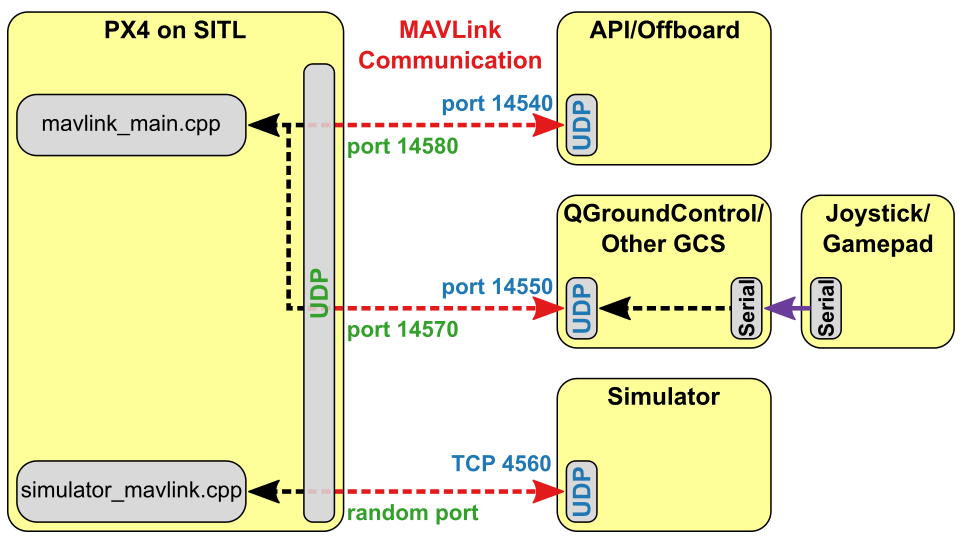
\includegraphics[width=0.8\textwidth]{picture/sitl.png}
    %   \caption{SITL}
    % \end{figure}
    % \begin{figure}[htbp]
    %   \centering
    %   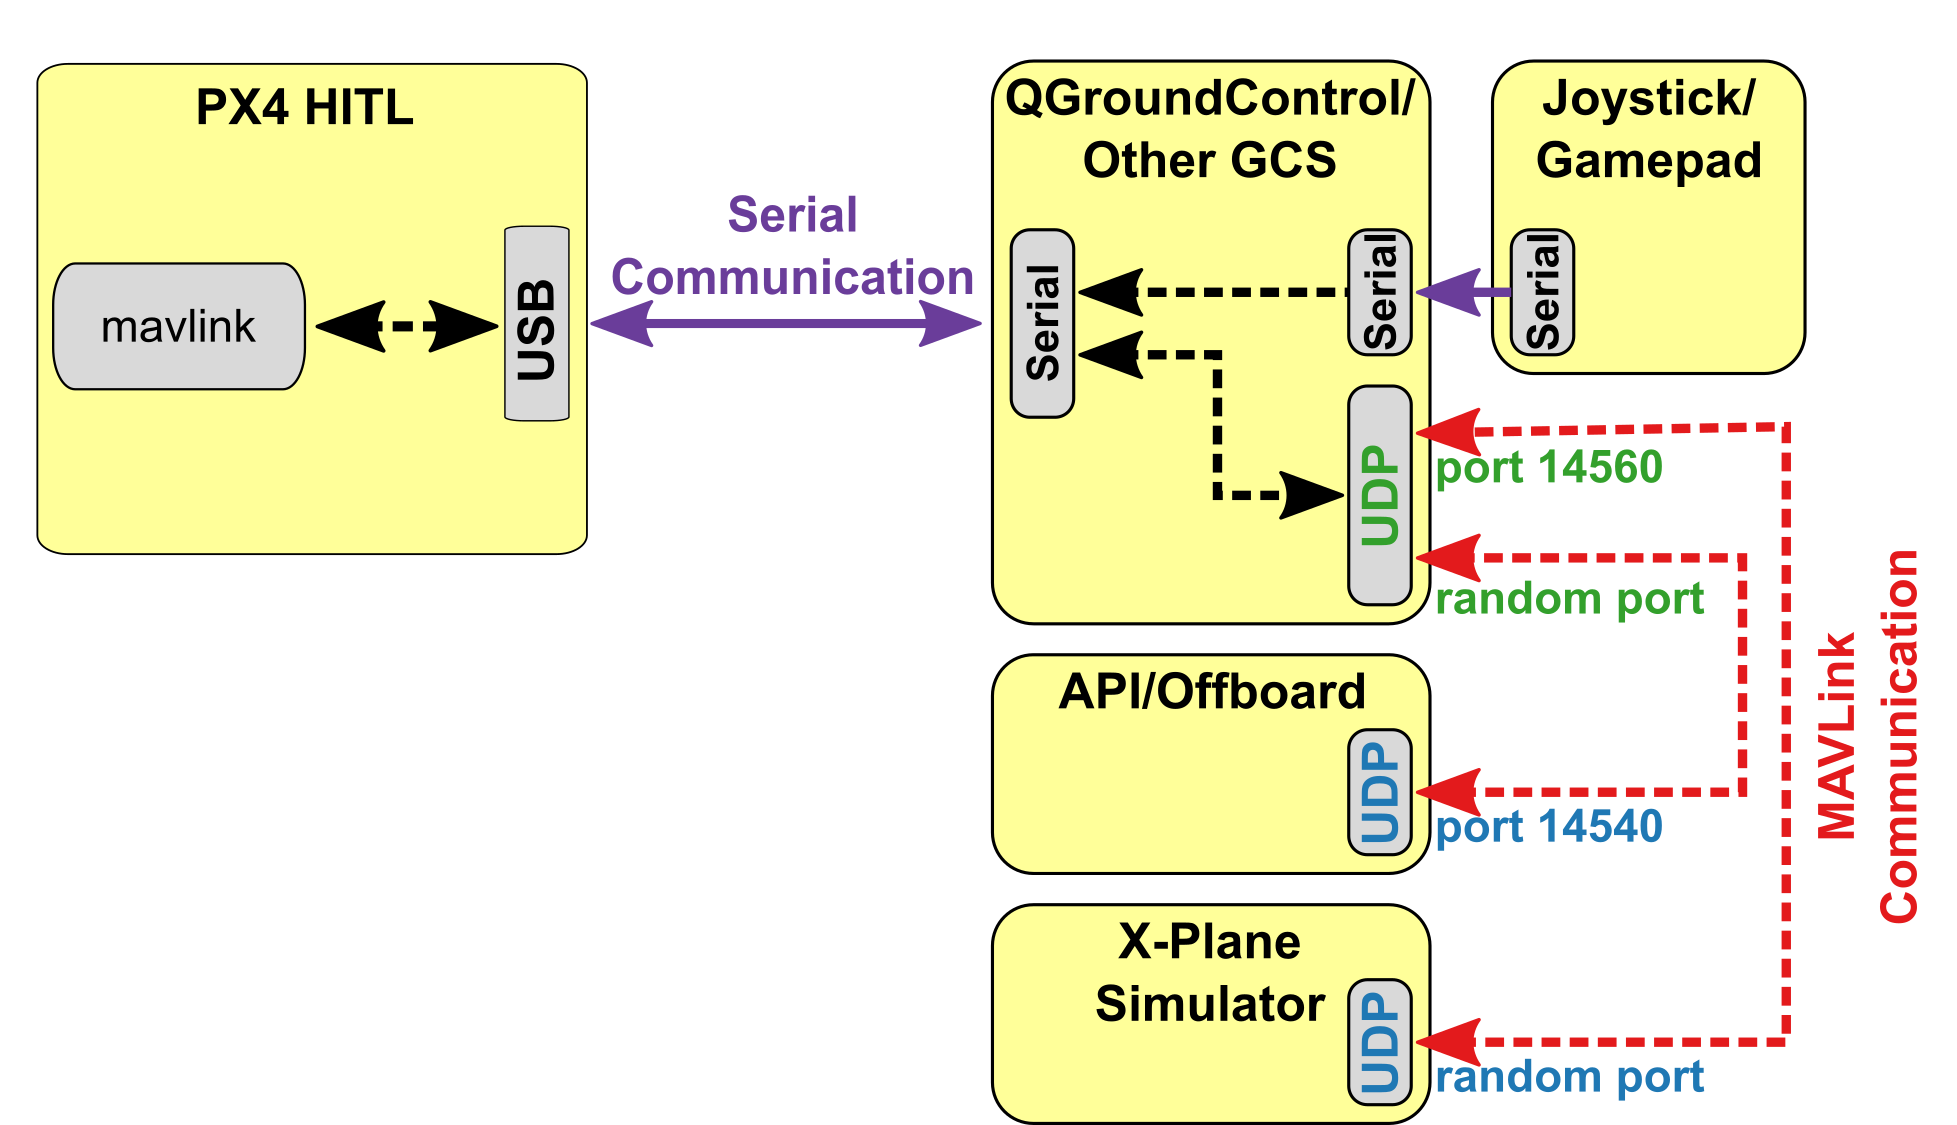
\includegraphics[width=0.8\textwidth]{picture/hitl.png}
    %   \caption{HITL-Xplane}
    % \end{figure}
    % \begin{figure}[htbp]
    %   \centering
    %   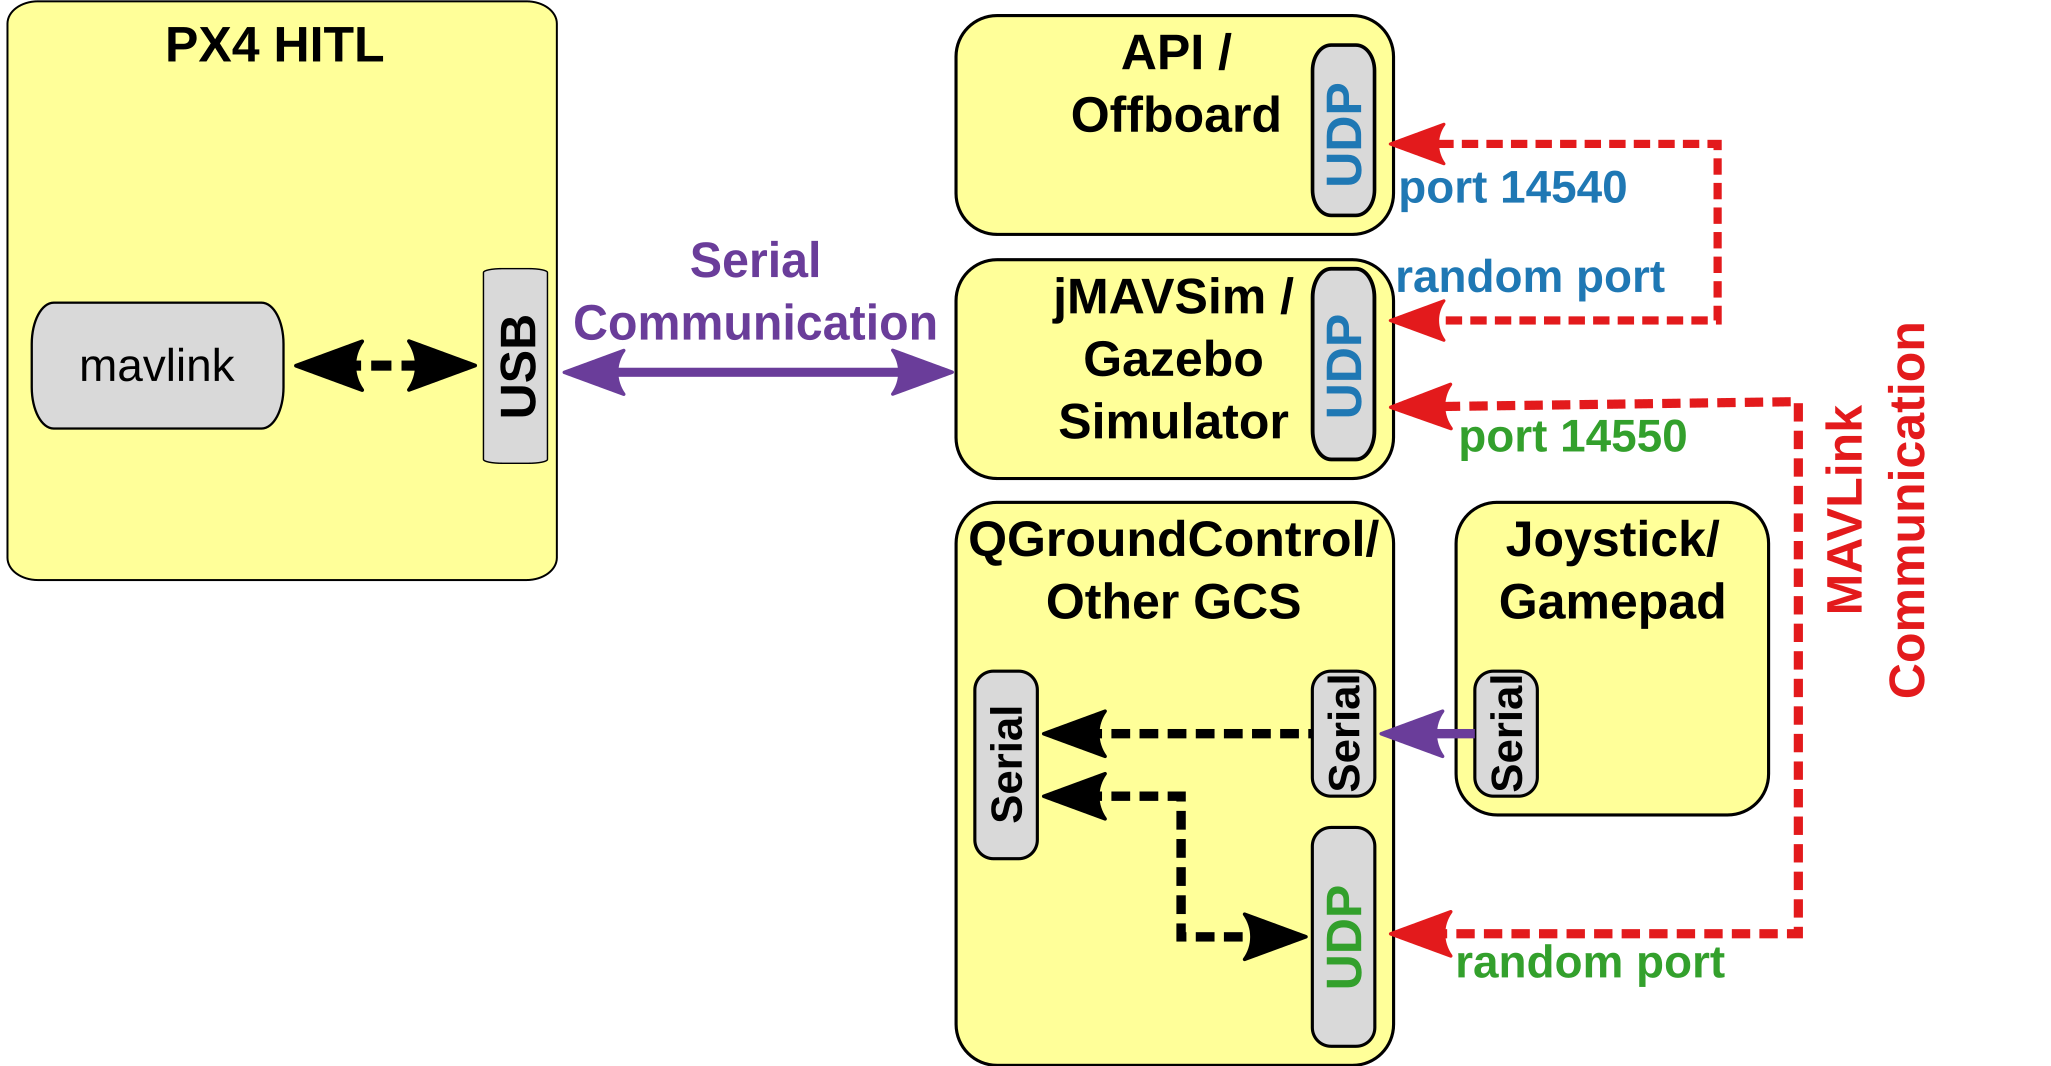
\includegraphics[width=0.8\textwidth]{picture/hitl2.png}
    %   \caption{HITL-Gazebo}
    % \end{figure}
    % \clearpage
    % \section{计算机视觉}
    %     整理一下当前的任务流.
    %   计算机视觉, 是一门研究如何对数字图像或视频进行高层语义理解的交叉学科, 赋予了机器"看"的能力, 需要实现人的大脑中(主要是视觉皮层区)的视觉能力. \par
    %   图像处理, 用计算机对图像进行分析, 已达到所需结果的技术. 图像处理一般指的是数字图像处理, 图像处理的技术一般包括图像压缩, 增强和复原, 匹配, 描述和识别三个部分. 
    %   \par 图像处理就是各种的图像变换处理, 计算机视觉在图像处理之后再识别其内部的语义, 理解视频流中的内容. 
    % \begin{figure}[htbp]
    %     \centering
    %     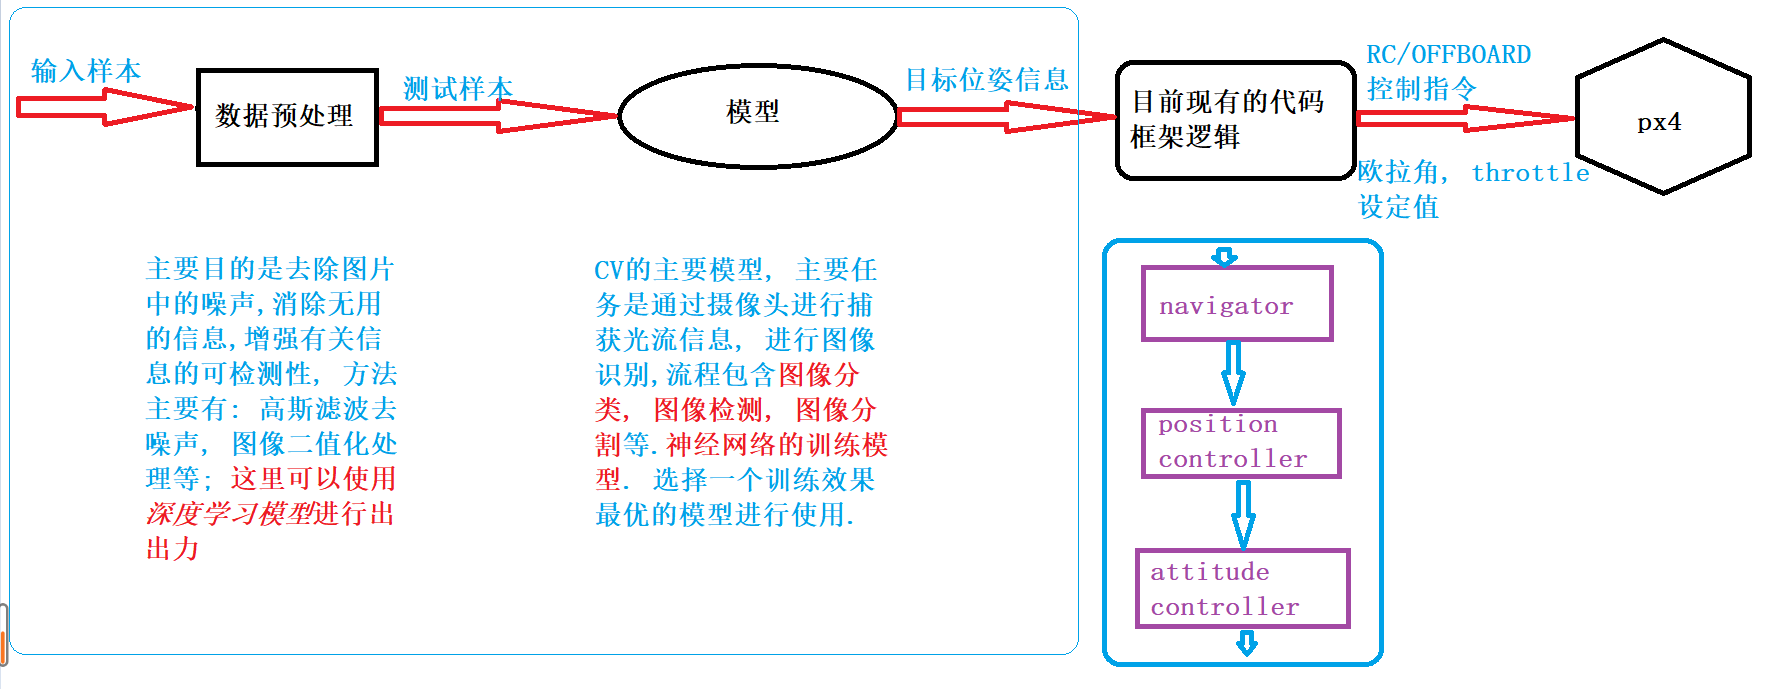
\includegraphics[width=0.8\textwidth]{picture/CV_Flow.png}
    %     \caption{CV数据流}
    % \end{figure}  
    % \clearpage
    % \section{算法内部}
    %     有时间的话细说一下代码
\end{document}

    \documentclass[UTF8,a4paper,10pt,nocolorlinks]{ctexart}
\usepackage[left=2.50cm, right=2.50cm, top=2.50cm, bottom=2.50cm]{geometry} %页边距
\CTEXsetup[format={\Large\bfseries}]{section} %设置章标题居左   
\usepackage{ctex}
\CTEXoptions[today=old]
\usepackage{cite}
% 代码块儿
\usepackage{textcomp} % 必须加上,否则报错
\usepackage{listings}
\usepackage{xcolor}
% \usepackage{fontspec}
% \setmonofont{Consolas}
\usepackage{varioref}       % ref 跨页调用
\usepackage{ctex}
\usepackage{multicol}
\usepackage{amssymb}        % 等于号 上面 加一个三角形
\usepackage{setspace}
\usepackage{tikz} % package used for the tikz
\usepackage{mdframed}
\usepackage{titletoc}
\usepackage{etoolbox}

\usepackage{helvet}
\usepackage{caption}
\usepackage{multicol} %用于实现在同一页中实现不同的分栏
\usepackage{changepage}
\usepackage{graphics}
\usepackage{amsmath, amsfonts, amssymb} % math equations, symbols
\usepackage[english]{babel}
\usepackage{color}      % color content
\usepackage{graphicx}   % import figures
\usepackage{url}        % hyperlinks
\usepackage{bm}         % bold type for equations
\usepackage{multirow}
\usepackage{booktabs}
\usepackage{epstopdf}
\usepackage{epsfig}
\usepackage{algorithm}
\usepackage{algorithmic}

\usepackage[pagestyles]{titlesec}
% \renewcommand{\algorithmicrequire}{ \textbf{Input:}}     % use Input in the format of Algorithm  
% \renewcommand{\algorithmicinput}{ \textbf{Input:}}     % use Input in the format of Algorithm  
\renewcommand{\algorithmicensure}{ \textbf{Input:}} % use Initialize in the format of Algorithm  
% \renewcommand{\algorithmicreturn}{ \textbf{Output:}}     % use Output in the format of Algorithm  
\renewcommand{\figurename}{图}
% 引用参考文献标号显示在右上角
\newcommand{\upcite}[1]{\textsuperscript{\textsuperscript{\cite{#1}}}}

\newpagestyle{teststyle}{
  \sethead{学号: 2019520941}{\sectiontitle}{第\thepage页}
  \renewcommand{\makeheadrule}{
    \makebox[0pt][l]{\rule[-.3\baselineskip]{\linewidth}{.5pt}}
    \rule[-.4\baselineskip]{\linewidth}{.5pt}
  }
}
\usepackage{color}
\usepackage{subfigure}
\usepackage{changepage}
\usepackage{fancyhdr} %设置页眉、页脚
\pagestyle{fancy}  %%%单线页眉
\fancyhead{}
\fancyhead[LO]{学习总结}
\fancyhead[RO]{冯学伟}
% \fancyfoot[RO]{\thepage}
\fancypagestyle{plain}{%
  \pagestyle{fancy}
}
\usepackage{shorttoc}
\usepackage{xcolor}
\usepackage{mdframed}
\usepackage{titletoc}
% \renewcommand{\today}{\CJKnumber\year 年 \CJKnumber\month 月 \CJKnumber\day 日}

\DeclareRobustCommand{\chuhao}{\fontsize{42pt}{\baselineskip}\selectfont}  % 初号
\DeclareRobustCommand{\xiaochu}{\fontsize{36pt}{\baselineskip}\selectfont} % 小初
\DeclareRobustCommand{\yihao}{\fontsize{26pt}{\baselineskip}\selectfont}   % 一号
\DeclareRobustCommand{\xiaoyi}{\fontsize{24pt}{\baselineskip}\selectfont}  % 小一
\DeclareRobustCommand{\erhao}{\fontsize{22pt}{\baselineskip}\selectfont}   % 二号
\DeclareRobustCommand{\xiaoer}{\fontsize{18pt}{\baselineskip}\selectfont}  % 小二
\DeclareRobustCommand{\sanhao}{\fontsize{16pt}{\baselineskip}\selectfont}  % 三号 
\DeclareRobustCommand{\xiaosan}{\fontsize{15pt}{\baselineskip}\selectfont} % 小三
\DeclareRobustCommand{\sihao}{\fontsize{14pt}{\baselineskip}\selectfont}   % 四号
\DeclareRobustCommand{\xiaosi}{\fontsize{12pt}{\baselineskip}\selectfont}  % 小四
\DeclareRobustCommand{\wuhao}{\fontsize{10.5pt}{\baselineskip}\selectfont} % 五号
\DeclareRobustCommand{\xiaowu}{\fontsize{9pt}{\baselineskip}\selectfont}   % 小五
\DeclareRobustCommand{\liuhao}{\fontsize{7.5pt}{\baselineskip}\selectfont} % 六号
\DeclareRobustCommand{\xiaoliu}{\fontsize{6.5pt}{\baselineskip}\selectfont}% 小六
\DeclareRobustCommand{\qihao}{\fontsize{5.5pt}{\baselineskip}\selectfont}  % 七号

\lstset{numbers=left,numberstyle=\tiny,
breaklines=true,  %代码过长则换行
keywordstyle=\color{blue!70},commentstyle=\color{red!50!green!50!blue!50},frame=shadowbox, rulesepcolor=\color{gray!20!green!20!blue!20},escapeinside=``,xleftmargin=2em,xrightmargin=2em, aboveskip=1em}

\providecommand{\keywords}[1]{\textbf{\textit{keywords---}} #1}

 
\usepackage{hyperref} %bookmarks
% \usepackage[colorlinks,linkcolor=red,anchorcolor=blue,citecolor=green,CJKbookmarks=True]{hyperref}
\hypersetup{colorlinks, bookmarks, unicode} % unicode
 
\captionsetup[figure]{labelfont={bf},labelformat={default},labelsep=period,name={图}}
\newenvironment{figurehere}
{\def\@captype{figure}}
{}

\title{
    \huge{\textbf{2020.07.07 第一次总结}}\\
}
\author{冯学伟}
\date{2020.07.07}

\begin{document}
    \maketitle
    % \renewcommand{\contentsname}{目录}  % 将Contents改为目录
    % \tableofcontents
    % \thispagestyle{empty} % 设置当前页 页版式
    
   
    本周计划: 
    \begin{itemize}
      \item 理论学习: 继续就那本书进行学习, 按照进度, 应该可以看一章多一点.
      \item 调bug: 将HITL调通
    \end{itemize}
    % \section{本周的学习总结}
    %     \subsection{chapter 3}
    %     本章, 主要介绍了刚体运动的运动学(kinematics)和动力学(dynamics); 其中主要定义了
    %     \begin{itemize}
    %       \item 位置和速度的关系(kinematics)
    %       \item 动力学表达式
    %       \item 12个状态量的表达式
    %     \end{itemize}
    %     首先介绍了\textcolor{red}{声明了MAV状态变量}, 12个, 
    %     其中, 和平移运动相关的三个位置变量(ned), 
    %     三个速度变量($u, v, \omega$, $i^{b}, j^{b}, k^{b}$), 
    %     三个角度(roll($F^{v2}$), pitch($F^{v1}$), yaw($F^{v}$)), 
    %     三个角速度($i^{b}, j^{b}, k^{b}$); 
    %     其次推导了\textcolor{red}{运动学, 即位置和速度的关系}, 
    %     我们需要将其从位置的导数即速度从体坐标系下转换到vehicle坐标系下进行计算.  
    %     因为位置是NED, 属于惯性坐标系下的值, 那么速度也是表示在惯性坐标系, 而惯性坐标系和vehicle坐标系三轴的指向是一样的, 唯一不一样的是二者的原点位置不同, 前者的原点位置是在地心, 后者是在MAV的质心, 且从体坐标系到vehicle存在确定的旋转矩阵, 故我们需要做这样的一个变换, 从而使其统一化;
    %     最后也推导了\textcolor{red}{动力学方程}, 针对牛顿第二定律的应用, 分别介绍了其在MAV的平移运动和旋转运动的动力学模型,
    %     \subsection{chapter 4}
    %     本章, 主要关注于力和力矩的梳理, 主要的来源是
    %     \begin{itemize}
    %       \item 重力(没有产生力矩)
    %       \item 空气动力($f_{a}, m_{a}$)
    %       \item 推力($f_{p}, m_{p}$)
    %       \item 大气的扰动, 即风速
    %     \end{itemize}
    %     关于重力, 推导出了其与欧拉角的数学关系式; 关于空气动力, 从纵向和横向两个方面进行了描述, 其中也介绍了无人机的控制平面, 包括 方向舵-副翼-升降舵无人机架构; 方向升降舵无人机架构; 升降翼舵无人机架构, 以及后二者和前者的转化关系式. 
    % \clearpage
    % \section{代码框架的梳理}
    %     结合框图来进行阐述
      
    % \clearpage
    % \section{simulation}
    % \begin{figure}[htbp]
    %   \centering
    %   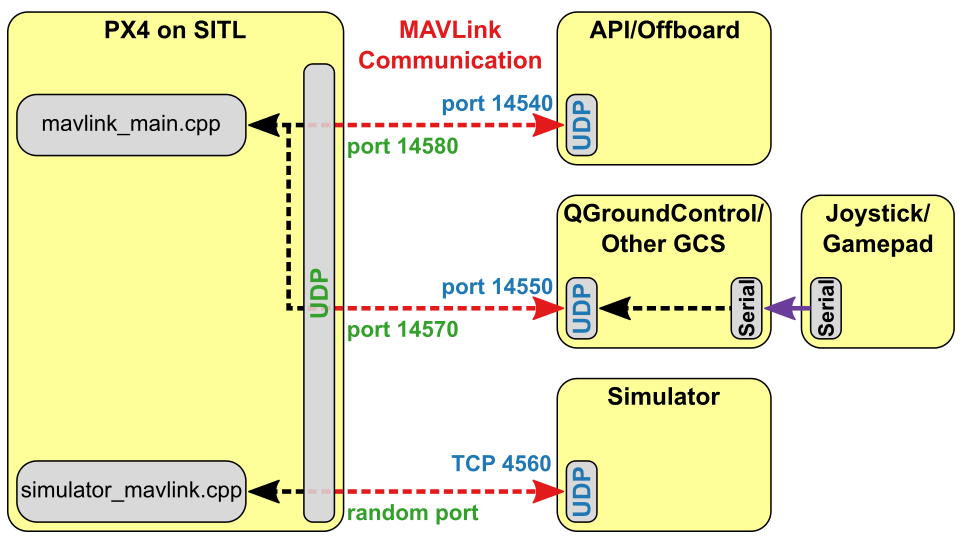
\includegraphics[width=0.8\textwidth]{picture/sitl.png}
    %   \caption{SITL}
    % \end{figure}
    % \begin{figure}[htbp]
    %   \centering
    %   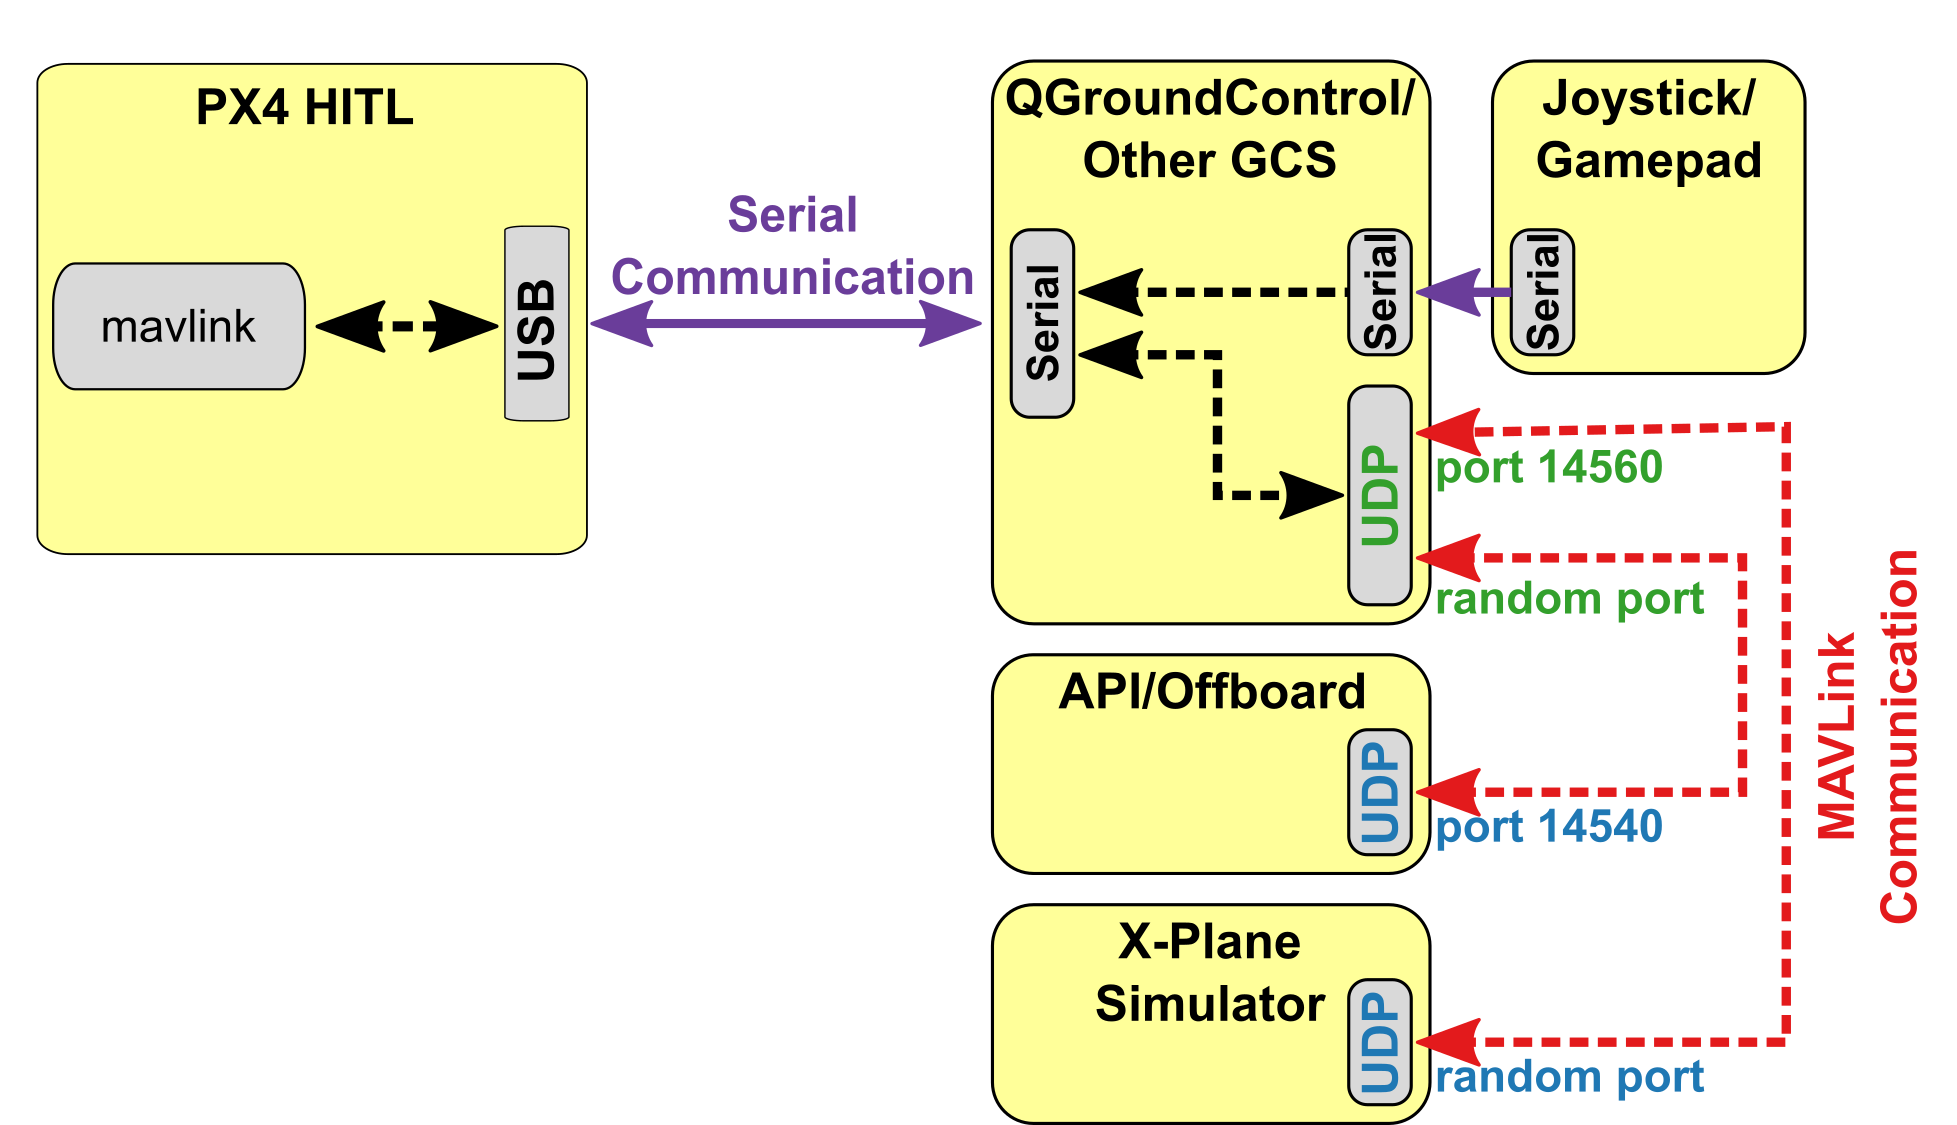
\includegraphics[width=0.8\textwidth]{picture/hitl.png}
    %   \caption{HITL-Xplane}
    % \end{figure}
    % \begin{figure}[htbp]
    %   \centering
    %   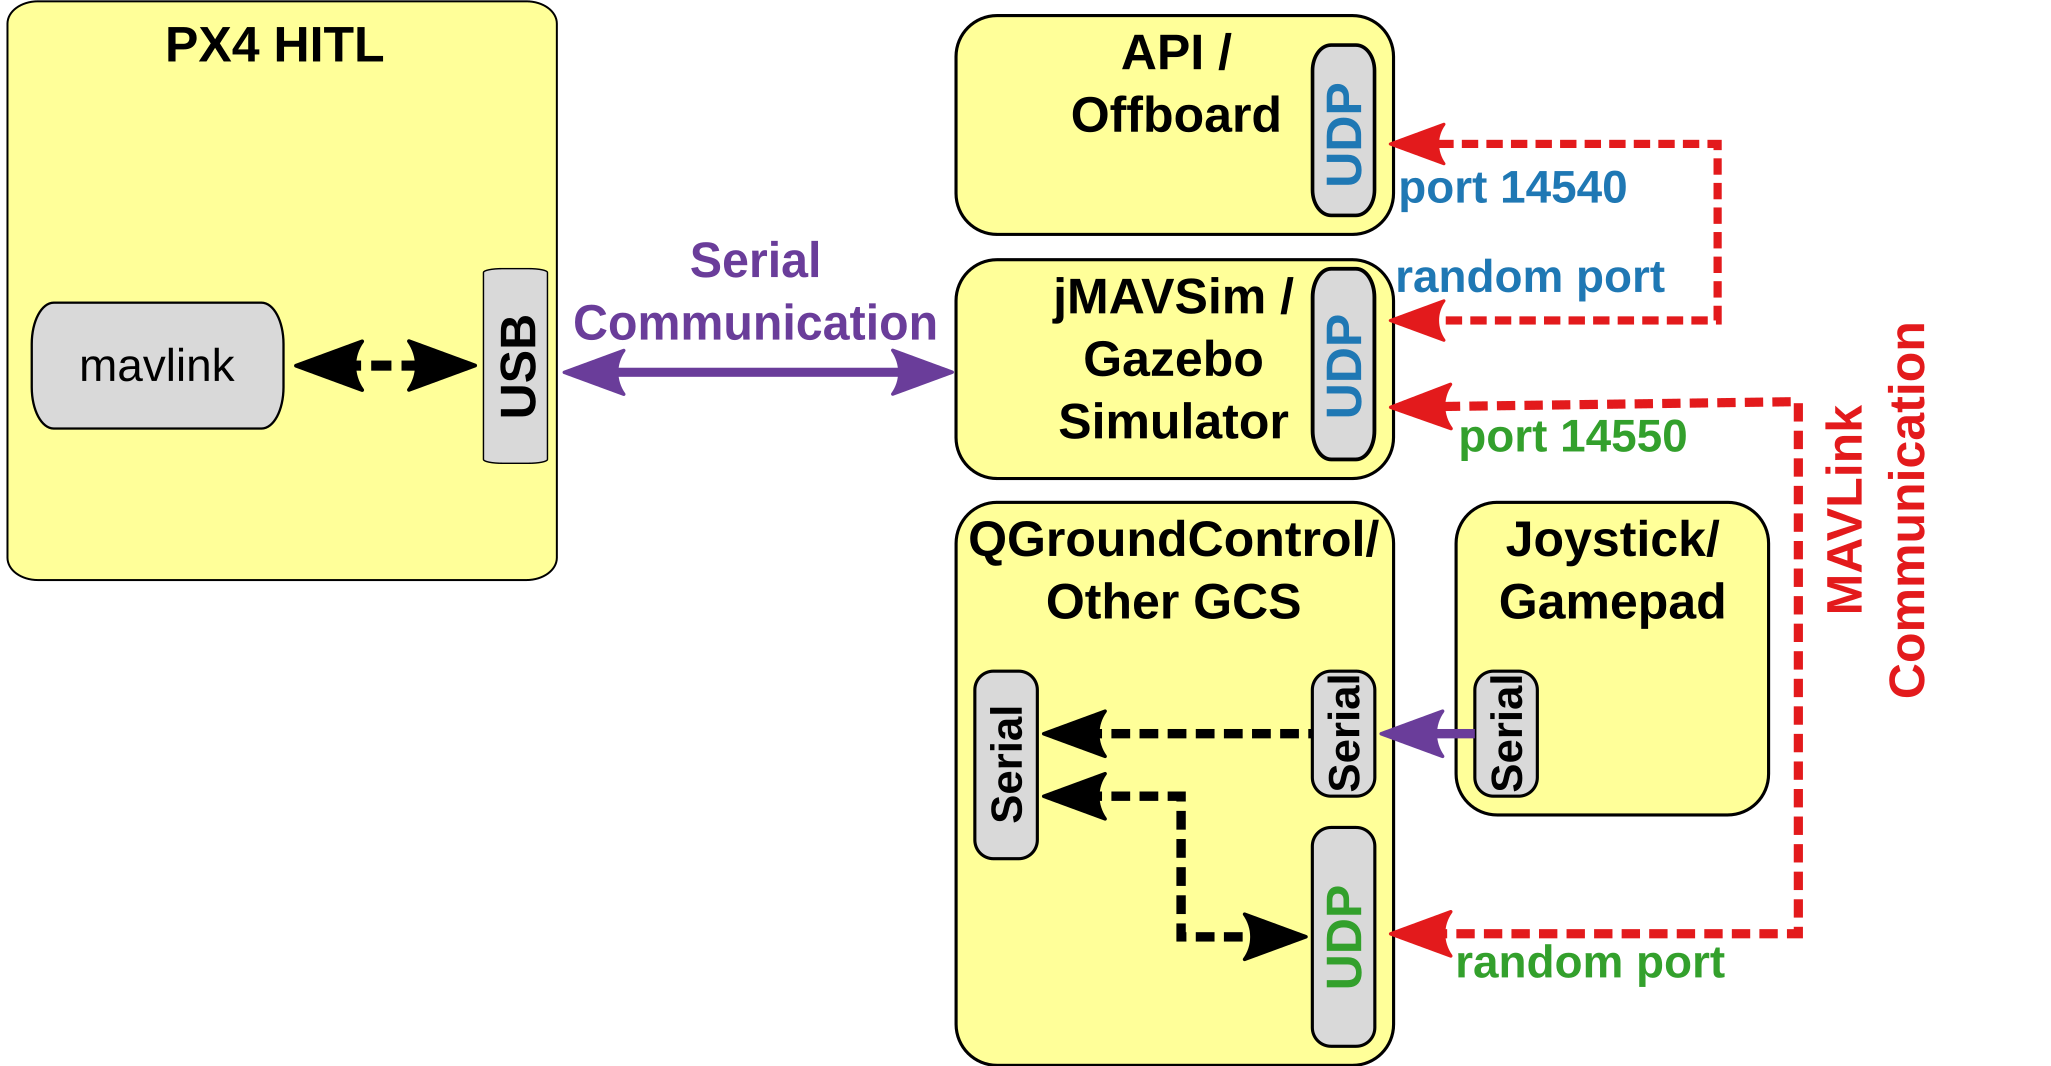
\includegraphics[width=0.8\textwidth]{picture/hitl2.png}
    %   \caption{HITL-Gazebo}
    % \end{figure}
    % \clearpage
    % \section{计算机视觉}
    %     整理一下当前的任务流.
    %   计算机视觉, 是一门研究如何对数字图像或视频进行高层语义理解的交叉学科, 赋予了机器"看"的能力, 需要实现人的大脑中(主要是视觉皮层区)的视觉能力. \par
    %   图像处理, 用计算机对图像进行分析, 已达到所需结果的技术. 图像处理一般指的是数字图像处理, 图像处理的技术一般包括图像压缩, 增强和复原, 匹配, 描述和识别三个部分. 
    %   \par 图像处理就是各种的图像变换处理, 计算机视觉在图像处理之后再识别其内部的语义, 理解视频流中的内容. 
    % \begin{figure}[htbp]
    %     \centering
    %     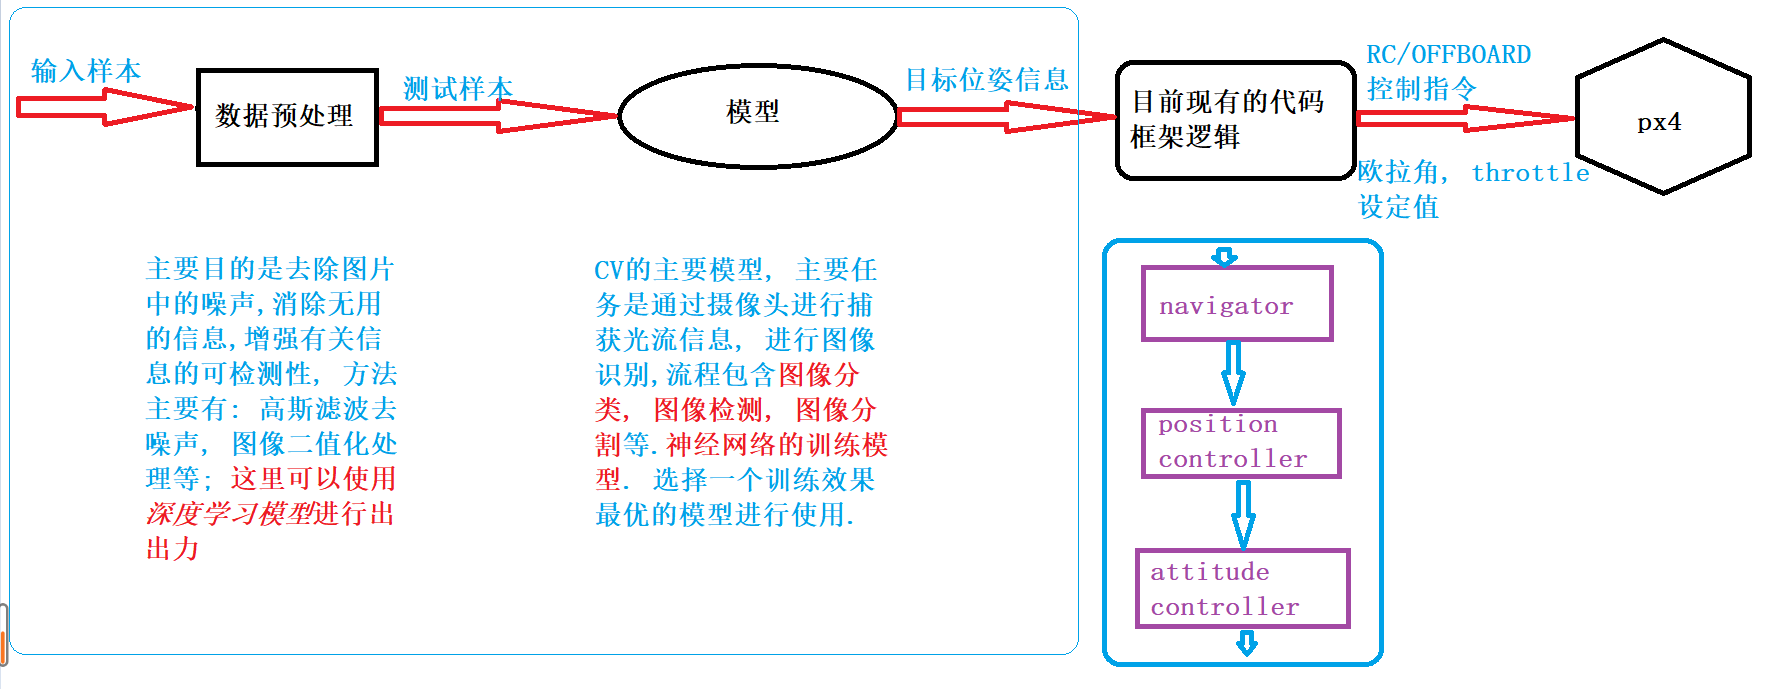
\includegraphics[width=0.8\textwidth]{picture/CV_Flow.png}
    %     \caption{CV数据流}
    % \end{figure}  
    % \clearpage
    % \section{算法内部}
    %     有时间的话细说一下代码
\end{document}

        \chapter{20200723}
    \section{20200723}
    \begin{itemize}
        \item[(1)] 给第一版加上了退出保护机制, 让其能退出 attitude controller , 从而将飞控的控制权交给qgc或者是Joystick. (详情可见~\ref{sec:protect})
        \item[(2)] 对offboard进行了bug调节 
        \item[(3)] 协调转弯 (\textcolor{red}{$\dot{\psi} = \frac{g}{V_{a}} tan \phi $}) (详情可见~\ref{sec:turn}).
    \end{itemize}
    \clearpage

    \section{The centrifugal force}
    当物体在做非直线运动时(非牛顿环境,例如:圆周运动或转弯运动),
    因物体一定有本身的质量存在,
    质量造成的惯性会强迫物体继续朝着运动轨迹的切线方向(原来那一瞬间前进的直线方向)前进,
    而非顺着接下来转弯过去的方向走。
    \par 若这个在做非直线运动的物体(例如:车)上有乘客的话,乘客由于同样随着车子做转弯运动,
    会受到车子向乘客提供的向心力,但是若以乘客为参照系,由于该参照系为非惯性系,
    他会受到与他相对静止的车子给他的一个指向圆心的向心力作用,
    但同时他也会给车子一个反向等大,由圆心指向外的力,就好像没有车子他就要被甩出去一样,这个力就是所谓的离心力。
    \section{concept}
    \begin{itemize}
        \item[(1)] 航向角是质心沿着速度方向在水平面上的投影与预定轨迹的切线方向之间的夹角, 记为$\chi$; \\ 偏航角是质心沿着机头方向在水平面上的投影与预定轨迹的切线方向之间的夹角, 记为 $\psi$.\\
        航向角$\chi$是地速相对于$i^{i}$(正北)方向的偏移角度, 偏航角$\psi$是空速方向; \\在没有风的情况下, 偏航角和航向角是相等的
        \item[(2)] 升力是垂直副翼向上的
        \item[(3)] roll的大小和方向: 机体坐标系OZb轴与通过机体OXb轴的铅垂面间的夹角,机体向右滚为正,反之为负。
        \item[(4)] $\gamma$是 地速方向和水平方向的夹角
        \item[(5)] 圆周运动的半径, 线速度, 以及角速度三者之间的关系: $v = r \omega$
    \end{itemize}
    \clearpage
    \setcounter{page}{1}        %从下面开始编页,页脚格式为导言部分设置的格式
    \section{退出保护机制}
    \label{sec:protect}
    当飞机进入到 ALTCTL 模式的时候, 退出保护机制会一直监控当前px4飞行模式是否有切换到其他模式的趋势, 即qgc或Joystick是否有争夺控制权的动作. 
    \begin{itemize}
      \item[(1)] 若有, 那么退出保护机制向 attitude controller 发送一个标志位, 来告知 attitude controller 不再发送 rc 控制指令. 进而退出 ALTCTL mode, 进入 RTL mode;
      \item[(2)] 若无, 那么一直监听.
    \end{itemize}
    \clearpage
    \section{Coordinated Turn 协调转弯}
    \label{sec:turn}
    方向角的变化率是和机体的roll以及倾斜角(bank angle)有关系, 我们需要寻找一个简单的关系来帮助我们研究这种线性传递函数的关系 -- 协调转弯. \par
    在协调转弯期间, 飞机在体坐标系下没有横向加速度. 从分析的角度来看, 协调转弯的一个假设运行我们得到一个简单的表达式将 heading rate 和 bank angle 联系起来. \par
    协调转弯时, 为了无人机没有侧向力, bank angle $\phi$ 被设置.
    在图\ref{fig:1}中, 作用在微型飞行器上的离心力与作用在水平方向上的升力的水平分量相等并相反。
    \begin{figure}[htpb]
        \centering
        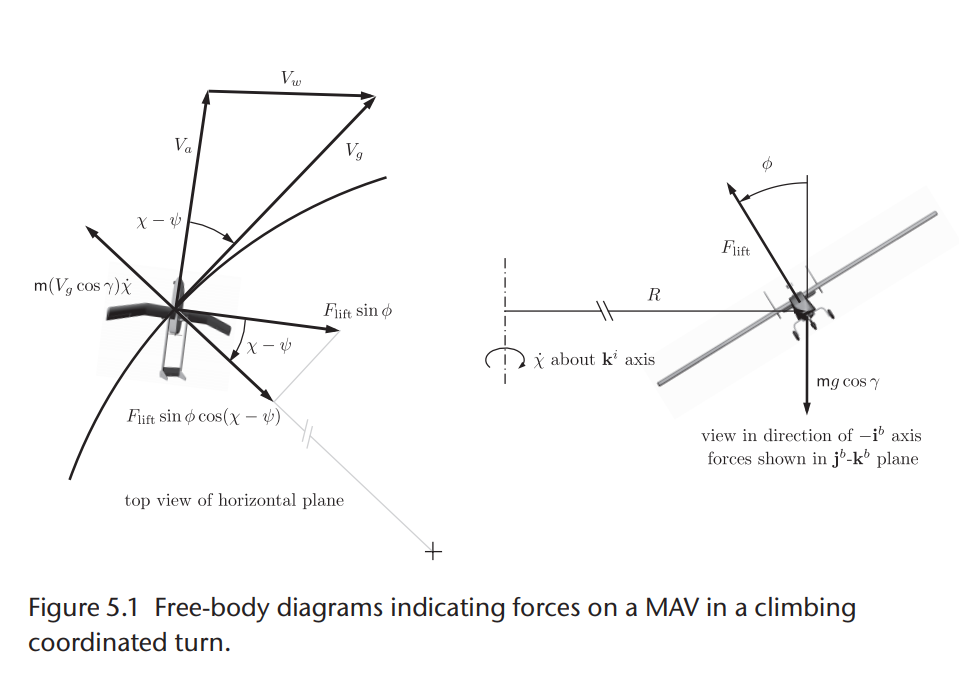
\includegraphics[width=0.8\textwidth]{pictures/chapter3/5_1.png}
        \caption{爬升协调转弯MAV上的力}
        \label{fig:1}
    \end{figure}
    \par 作用在水平方向力的关系表示如下: 
    \begin{align}
        F_{lift} sin \phi cos (\chi - \psi) &= m \frac{v^{2}}{R} \nonumber \\
        &= m v \omega \nonumber \\
        &= m (V_{g} cos \gamma) \dot{\chi} 
        \label{equ:1}
    \end{align}
    其中, $F_{lift}$代表的是升力, $\gamma$ 代表的是飞行轨迹的角度, $V_{g}, \chi$ 分别表示的是地速度以及方向角. \textcolor{red}{向心加速度的表达式: $a_{n} = \frac{v^{2}}{R} = v \omega$}
    \par 离心力(The centrifugal force)(\textcolor{red}{$m (V_{g} cos \gamma) \dot{\chi} $})计算的时候, 用到了在惯性坐标系$k^{i}$上的方向角变化率$\dot{\chi}$ 和 速度的水平分量 $V_{a}cos \gamma$
    \par 同样, 升力的垂直分量与重力在 $j^{b} - k^{b}$平面上的投影是等大反向的. 
    垂直方向上的合力为:
    \begin{equation}
        F_{lift} cos \phi = mg cos\gamma
        \label{equ:2}
    \end{equation}
    将等式\ref{equ:1}除以\ref{equ:2}得的 $\dot{\chi}$
    \begin{equation}
        \dot{\chi} = \frac{g}{V_{g}} tan \phi cos(\chi - \psi)
        \label{equ:3}
    \end{equation}
    等式\ref{equ:3}就是协调转弯的表达式. 
    \par 考虑到转弯半径等于 \textcolor{blue}{ $R = V_{g} \frac{cos \gamma}{\dot{\chi}}$}, 将上式代入半径中, 得到式子\ref{equ:4}. 在没有风或侧滑的情况下, 有\textcolor{red}{$V_{a} = V_{g}$和$\psi = \chi$}, 从而得到了式子\ref{equ:5}. 
    \begin{equation}
        R = \frac{V_{g}^{2} cos \gamma}{g tan \phi cos(\chi - \psi)} 
        \label{equ:4}
    \end{equation}
    \begin{equation}
        \dot{\chi} = \frac{g}{V_{g}} tan \phi = \dot{\psi} = \frac{g}{V_{a}} tan \phi
        \label{equ:5}
    \end{equation}
    \par 在 9.2 节中, 我们将要介绍 在有风的情况下 \textcolor{blue}{$ \dot{\psi} = \frac{g}{V_{a}} tan \phi$} 该式子也成立
    \clearpage
    \section{Kinematic Model of Controlled Flight}
    % 控制飞行动力学模型\par
    % 在推导降阶表达式中, 简化的目的是估计运动中力平衡以及动量平衡的关系式(这些包含了 $\dot{u}, \dot{v}, \dot{\omega}, \dot{p}, , \dot{q}, \dot{r}$), 预估这些变量需要计算复杂的空气动力. 这些变量表达式可以被更简单的动力学表达式替代. 
    % 这个更简单的动力学表达式是\textcolor{blue}{针对协调转弯和加速爬升的特定飞行条件而导出}.
    \begin{figure}[htpb]
        \centering
        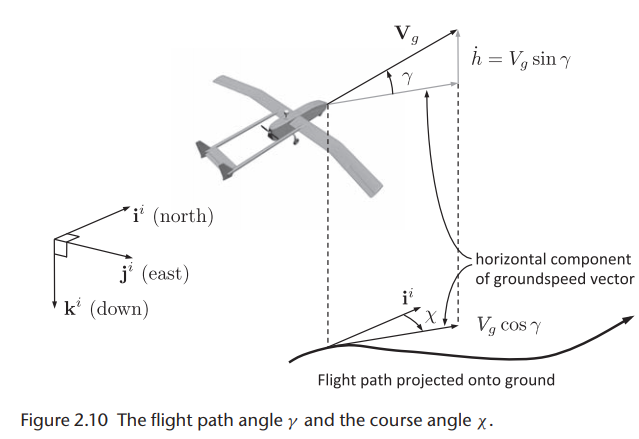
\includegraphics[width=0.8\textwidth]{pictures/chapter3/2_10.png}
        \caption{航线轨迹角度$\gamma$和航向角$\chi$}
        \label{fig:2_10}
    \end{figure}
    针对图\ref{fig:2_10}, 飞机相对于惯性系的速度矢量可以用航向角和(惯性参考)飞行路径角表示为 
    \begin{gather} % 输入多行公式
        V_{g}^{i} = V_{g} \begin{pmatrix}
            cos \chi cos \gamma \\
            sin \chi cos \gamma \\
            -sin \gamma \\
          \end{pmatrix}
          = \begin{pmatrix}
            \dot{p_{n}} \\
            \dot{p_{e}} \\
            \dot{h} \\
          \end{pmatrix}
          \label{equ:6}
      \end{gather}
    \par 由于控制飞机的航向和空速是很常见的,因此用$\psi$和$V_{a}$表示等式\ref{equ:6}很有用. 
    \begin{gather} % 输入多行公式
        V_{g} \begin{pmatrix}
            cos \chi cos \gamma \\
            sin \chi cos \gamma \\
            -sin \gamma \\
          \end{pmatrix} - \begin{pmatrix}
            w_{n} \\
            w_{e} \\
            w_{d} \\
          \end{pmatrix} =  V_{a} \begin{pmatrix}
            cos \psi cos \gamma_{a} \\
            sin \psi cos \gamma_{a} \\
            -sin \gamma_{a} \\
          \end{pmatrix}
          \label{equ:wind}
      \end{gather}
      结合风的表达式\ref{equ:wind}(地速等于空速加风速, 
        其中的 $\gamma_{a}$ 代表的是 空速的方向和水平方向的夹角), 我们可以得到
      \begin{gather} % 输入多行公式
        \begin{pmatrix}
            \dot{p_{n}} \\
            \dot{p_{e}} \\
            \dot{h} \\
          \end{pmatrix} = V_{a} \begin{pmatrix}
            cos \psi cos \gamma_{a} \\
            sin \psi cos \gamma_{a} \\
            sin \gamma_{a} \\
          \end{pmatrix} +  \begin{pmatrix}
            w_{n} \\
            w_{e} \\
            -w_{d} \\
          \end{pmatrix}
          \label{equ:7}
      \end{gather}
      如果我们假设飞机保持在一个恒定的高度,并且没有向下的风分量,那么运动学表达式简化为\ref{equ:8}, 同样该模型也是无人机领域中比较常用的模型. 
      \begin{gather} % 输入多行公式
        \begin{pmatrix}
            \dot{p_{n}} \\
            \dot{p_{e}} \\
            \dot{h} \\
          \end{pmatrix} = V_{a} \begin{pmatrix}
            cos \psi \\
            sin \psi \\
            0 \\
          \end{pmatrix} +  \begin{pmatrix}
            w_{n} \\
            w_{e} \\
            0 \\
          \end{pmatrix}
          \label{equ:8}
      \end{gather}
      \subsection{Coordinated Turn}
      之前的协调转弯的表达式为 $\dot{\chi} = \frac{g}{V_{g}} tan \phi cos(\chi - \psi)$. 
      即使在第6章中描述的自动驾驶回路并没有强制执行协调转弯条件,
      飞机必须倾斜才能转弯(而不是打滑才能转弯)这个基本条件已经被这个模型捕捉到了。\par
      协调转弯可以被 heading 和 空速进行表示. 我们先对\ref{equ:wind}两边进行求导, 得到下面的式子\ref{equ:9}
      \begin{gather} % 输入多行公式
        \begin{pmatrix}
            cos \chi cos \gamma & - V_{g} sin \chi cos \gamma & - V_{g} cos \chi sin \gamma \\
            sin \chi cos \gamma & V_{g} cos \chi cos \gamma & - V_{g} sin \chi sin \gamma \\
            -sin \gamma & 0 & -cos \gamma \\
          \end{pmatrix} \begin{pmatrix}
            \dot{V_{g}} \\
            \dot{\chi} \\
            \dot{\gamma} \\
        \end{pmatrix}
          = \begin{pmatrix}
            cos \psi cos \gamma_{a} & - V_{a} sin \psi cos \gamma_{a} & - V_{a} cos \psi sin \gamma_{a} \\
            sin \psi cos \gamma_{a} & V_{a} cos \psi cos \gamma_{a} & - V_{a} sin \psi sin \gamma_{a} \\
            -sin \gamma_{a} & 0 & -cos \gamma_{a} \\
          \end{pmatrix} \begin{pmatrix}
            \dot{V_{a}} \\
            \dot{\psi} \\
            \dot{\gamma_{a}} \\
        \end{pmatrix}
          \label{equ:9}
      \end{gather}
      \par 在定高和没有向下风分量的情况下, $\gamma, \gamma_{a}, \dot{\gamma}, \dot{\gamma_a}$ 和 $w_{d}$ 都是0, 根据$\dot{V_{a}}$ 和$\dot{\chi}$求解$\dot{V_{g}}$ 和$\dot{\psi}$
      \begin{equation}
        \begin{split}
          \dot{V_{g}} &= \frac{\dot{V_{a}}}{cos (\chi - \psi)} + V_{g} \dot{\chi} tan(\chi - \psi) \\
          \dot{\psi} &= \frac{\dot{V_{a}}}{V_{a}} tan (\chi - \psi) + \frac{V_{g} \dot{\chi}}{V_{a}cos(\chi - \psi)}
        \end{split}
    \end{equation}
    \par 若假定空速为常数, 那么得\ref{equ:10} 最值得注意的是在有风的情况下,这个等式是成立的。
    \begin{equation}
        \dot{\chi} = \frac{g}{V_{g}} tan \phi 
        \label{equ:10}
    \end{equation}
    \subsection{Accelerating Climb}
% \end{document}
    % \chapter{introduce}
\section{引言}
        \begin{itemize}
            \item 本课题研究背景
            \item 本课题研究前景
            \item 本课题知识难点
            \item 本课题结构罗列
        \end{itemize}
    % \chapter{controllers}
\section{无人机控制器}
无人机总的概述 \dots.
\begin{itemize}
    \item 无人机三大控制器介绍
    \item 无人机内部控制器数据流走向
\end{itemize}
    %     \chapter{landingLogical}
    \section{飞行器着陆原理分析}   
    通常的基础方法,      
    \begin{itemize}
        \item 光流场, 三个阶段
        \item 横向控制
        \item 纵向控制
    \end{itemize}
    %     \chapter{visionGuidence}
    
    \section{无人机视觉引导}
        \subsection{视觉体系结构}
            \begin{itemize}
                \item 视觉体系结构阐述
                \item 视觉数据流走向
            \end{itemize}
    % % 前面的都是基础知识, 方法, 只是介绍, 以及各自的优点和缺点, 我需要解决的问题, 每一章都说一个缺点, 在后面 针对上面的缺点进行解决

    %     \chapter{visionGuidence}
    
    \section{融合}
    若内容太多, 继续拆分 \\
    数学模式 方法 公式推导, 可以对应的说(分节), 也可以整合到一起, 看内容的多少
    \par 传感器选择
    \par 横向控制
    \par 纵向控制
    \par 引导算法
    %     \chapter{simulations}
    
    \section{仿真平台的搭建}
        
        这个不太了解\dots.
        
        目前还是需要多看, 多了解. 
    % \documentclass[UTF8,a4paper,10pt,nocolorlinks]{ctexart}
\usepackage[left=2.50cm, right=2.50cm, top=2.50cm, bottom=2.50cm]{geometry} %页边距
\CTEXsetup[format={\Large\bfseries}]{section} %设置章标题居左   
\usepackage{ctex}
\CTEXoptions[today=old]
\usepackage{cite}
% 代码块儿
\usepackage{textcomp} % 必须加上,否则报错
\usepackage{listings}
\usepackage{xcolor}
% \usepackage{fontspec}
% \setmonofont{Consolas}
\usepackage{varioref}       % ref 跨页调用
\usepackage{ctex}
\usepackage{multicol}
\usepackage{amssymb}        % 等于号 上面 加一个三角形
\usepackage{setspace}
\usepackage{tikz} % package used for the tikz
\usepackage{mdframed}
\usepackage{titletoc}
\usepackage{etoolbox}

\usepackage{helvet}
\usepackage{caption}
\usepackage{multicol} %用于实现在同一页中实现不同的分栏
\usepackage{changepage}
\usepackage{graphics}
\usepackage{amsmath, amsfonts, amssymb} % math equations, symbols
\usepackage[english]{babel}
\usepackage{color}      % color content
\usepackage{graphicx}   % import figures
\usepackage{url}        % hyperlinks
\usepackage{bm}         % bold type for equations
\usepackage{multirow}
\usepackage{booktabs}
\usepackage{epstopdf}
\usepackage{epsfig}
\usepackage{algorithm}
\usepackage{algorithmic}

\usepackage[pagestyles]{titlesec}
% \renewcommand{\algorithmicrequire}{ \textbf{Input:}}     % use Input in the format of Algorithm  
% \renewcommand{\algorithmicinput}{ \textbf{Input:}}     % use Input in the format of Algorithm  
\renewcommand{\algorithmicensure}{ \textbf{Input:}} % use Initialize in the format of Algorithm  
% \renewcommand{\algorithmicreturn}{ \textbf{Output:}}     % use Output in the format of Algorithm  
\renewcommand{\figurename}{图}
% 引用参考文献标号显示在右上角
\newcommand{\upcite}[1]{\textsuperscript{\textsuperscript{\cite{#1}}}}

\newpagestyle{teststyle}{
  \sethead{学号: 2019520941}{\sectiontitle}{第\thepage页}
  \renewcommand{\makeheadrule}{
    \makebox[0pt][l]{\rule[-.3\baselineskip]{\linewidth}{.5pt}}
    \rule[-.4\baselineskip]{\linewidth}{.5pt}
  }
}
\usepackage{color}
\usepackage{subfigure}
\usepackage{changepage}
\usepackage{fancyhdr} %设置页眉、页脚
\pagestyle{fancy}  %%%单线页眉
\fancyhead{}
\fancyhead[LO]{学习总结}
\fancyhead[RO]{冯学伟}
% \fancyfoot[RO]{\thepage}
\fancypagestyle{plain}{%
  \pagestyle{fancy}
}
\usepackage{shorttoc}
\usepackage{xcolor}
\usepackage{mdframed}
\usepackage{titletoc}
% \renewcommand{\today}{\CJKnumber\year 年 \CJKnumber\month 月 \CJKnumber\day 日}

\DeclareRobustCommand{\chuhao}{\fontsize{42pt}{\baselineskip}\selectfont}  % 初号
\DeclareRobustCommand{\xiaochu}{\fontsize{36pt}{\baselineskip}\selectfont} % 小初
\DeclareRobustCommand{\yihao}{\fontsize{26pt}{\baselineskip}\selectfont}   % 一号
\DeclareRobustCommand{\xiaoyi}{\fontsize{24pt}{\baselineskip}\selectfont}  % 小一
\DeclareRobustCommand{\erhao}{\fontsize{22pt}{\baselineskip}\selectfont}   % 二号
\DeclareRobustCommand{\xiaoer}{\fontsize{18pt}{\baselineskip}\selectfont}  % 小二
\DeclareRobustCommand{\sanhao}{\fontsize{16pt}{\baselineskip}\selectfont}  % 三号 
\DeclareRobustCommand{\xiaosan}{\fontsize{15pt}{\baselineskip}\selectfont} % 小三
\DeclareRobustCommand{\sihao}{\fontsize{14pt}{\baselineskip}\selectfont}   % 四号
\DeclareRobustCommand{\xiaosi}{\fontsize{12pt}{\baselineskip}\selectfont}  % 小四
\DeclareRobustCommand{\wuhao}{\fontsize{10.5pt}{\baselineskip}\selectfont} % 五号
\DeclareRobustCommand{\xiaowu}{\fontsize{9pt}{\baselineskip}\selectfont}   % 小五
\DeclareRobustCommand{\liuhao}{\fontsize{7.5pt}{\baselineskip}\selectfont} % 六号
\DeclareRobustCommand{\xiaoliu}{\fontsize{6.5pt}{\baselineskip}\selectfont}% 小六
\DeclareRobustCommand{\qihao}{\fontsize{5.5pt}{\baselineskip}\selectfont}  % 七号

\lstset{numbers=left,numberstyle=\tiny,
breaklines=true,  %代码过长则换行
keywordstyle=\color{blue!70},commentstyle=\color{red!50!green!50!blue!50},frame=shadowbox, rulesepcolor=\color{gray!20!green!20!blue!20},escapeinside=``,xleftmargin=2em,xrightmargin=2em, aboveskip=1em}

\providecommand{\keywords}[1]{\textbf{\textit{keywords---}} #1}

 
\usepackage{hyperref} %bookmarks
% \usepackage[colorlinks,linkcolor=red,anchorcolor=blue,citecolor=green,CJKbookmarks=True]{hyperref}
\hypersetup{colorlinks, bookmarks, unicode} % unicode
 
\captionsetup[figure]{labelfont={bf},labelformat={default},labelsep=period,name={图}}
\newenvironment{figurehere}
{\def\@captype{figure}}
{}

\title{
    \huge{\textbf{2020.07.07 第一次总结}}\\
}
\author{冯学伟}
\date{2020.07.07}

\begin{document}
    \maketitle
    % \renewcommand{\contentsname}{目录}  % 将Contents改为目录
    % \tableofcontents
    % \thispagestyle{empty} % 设置当前页 页版式
    
   
    本周计划: 
    \begin{itemize}
      \item 理论学习: 继续就那本书进行学习, 按照进度, 应该可以看一章多一点.
      \item 调bug: 将HITL调通
    \end{itemize}
    % \section{本周的学习总结}
    %     \subsection{chapter 3}
    %     本章, 主要介绍了刚体运动的运动学(kinematics)和动力学(dynamics); 其中主要定义了
    %     \begin{itemize}
    %       \item 位置和速度的关系(kinematics)
    %       \item 动力学表达式
    %       \item 12个状态量的表达式
    %     \end{itemize}
    %     首先介绍了\textcolor{red}{声明了MAV状态变量}, 12个, 
    %     其中, 和平移运动相关的三个位置变量(ned), 
    %     三个速度变量($u, v, \omega$, $i^{b}, j^{b}, k^{b}$), 
    %     三个角度(roll($F^{v2}$), pitch($F^{v1}$), yaw($F^{v}$)), 
    %     三个角速度($i^{b}, j^{b}, k^{b}$); 
    %     其次推导了\textcolor{red}{运动学, 即位置和速度的关系}, 
    %     我们需要将其从位置的导数即速度从体坐标系下转换到vehicle坐标系下进行计算.  
    %     因为位置是NED, 属于惯性坐标系下的值, 那么速度也是表示在惯性坐标系, 而惯性坐标系和vehicle坐标系三轴的指向是一样的, 唯一不一样的是二者的原点位置不同, 前者的原点位置是在地心, 后者是在MAV的质心, 且从体坐标系到vehicle存在确定的旋转矩阵, 故我们需要做这样的一个变换, 从而使其统一化;
    %     最后也推导了\textcolor{red}{动力学方程}, 针对牛顿第二定律的应用, 分别介绍了其在MAV的平移运动和旋转运动的动力学模型,
    %     \subsection{chapter 4}
    %     本章, 主要关注于力和力矩的梳理, 主要的来源是
    %     \begin{itemize}
    %       \item 重力(没有产生力矩)
    %       \item 空气动力($f_{a}, m_{a}$)
    %       \item 推力($f_{p}, m_{p}$)
    %       \item 大气的扰动, 即风速
    %     \end{itemize}
    %     关于重力, 推导出了其与欧拉角的数学关系式; 关于空气动力, 从纵向和横向两个方面进行了描述, 其中也介绍了无人机的控制平面, 包括 方向舵-副翼-升降舵无人机架构; 方向升降舵无人机架构; 升降翼舵无人机架构, 以及后二者和前者的转化关系式. 
    % \clearpage
    % \section{代码框架的梳理}
    %     结合框图来进行阐述
      
    % \clearpage
    % \section{simulation}
    % \begin{figure}[htbp]
    %   \centering
    %   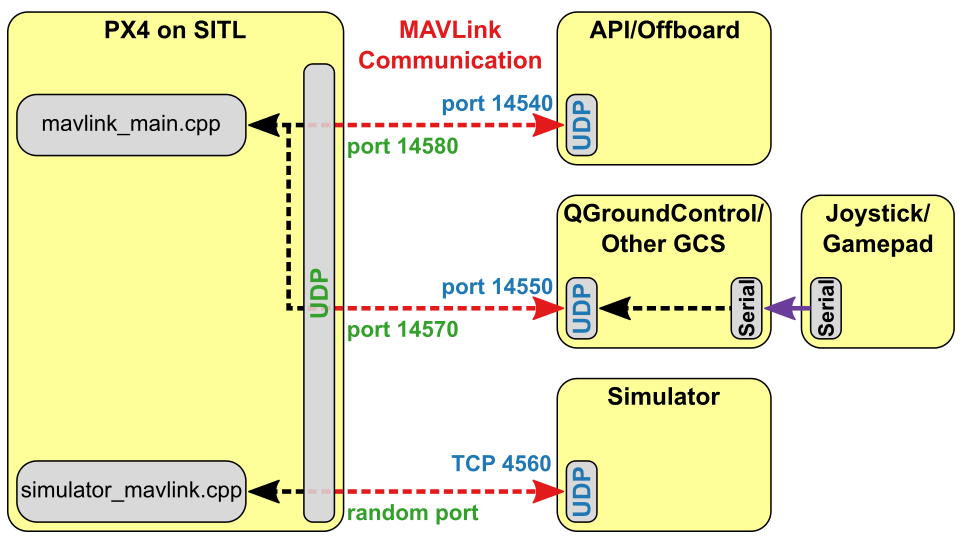
\includegraphics[width=0.8\textwidth]{picture/sitl.png}
    %   \caption{SITL}
    % \end{figure}
    % \begin{figure}[htbp]
    %   \centering
    %   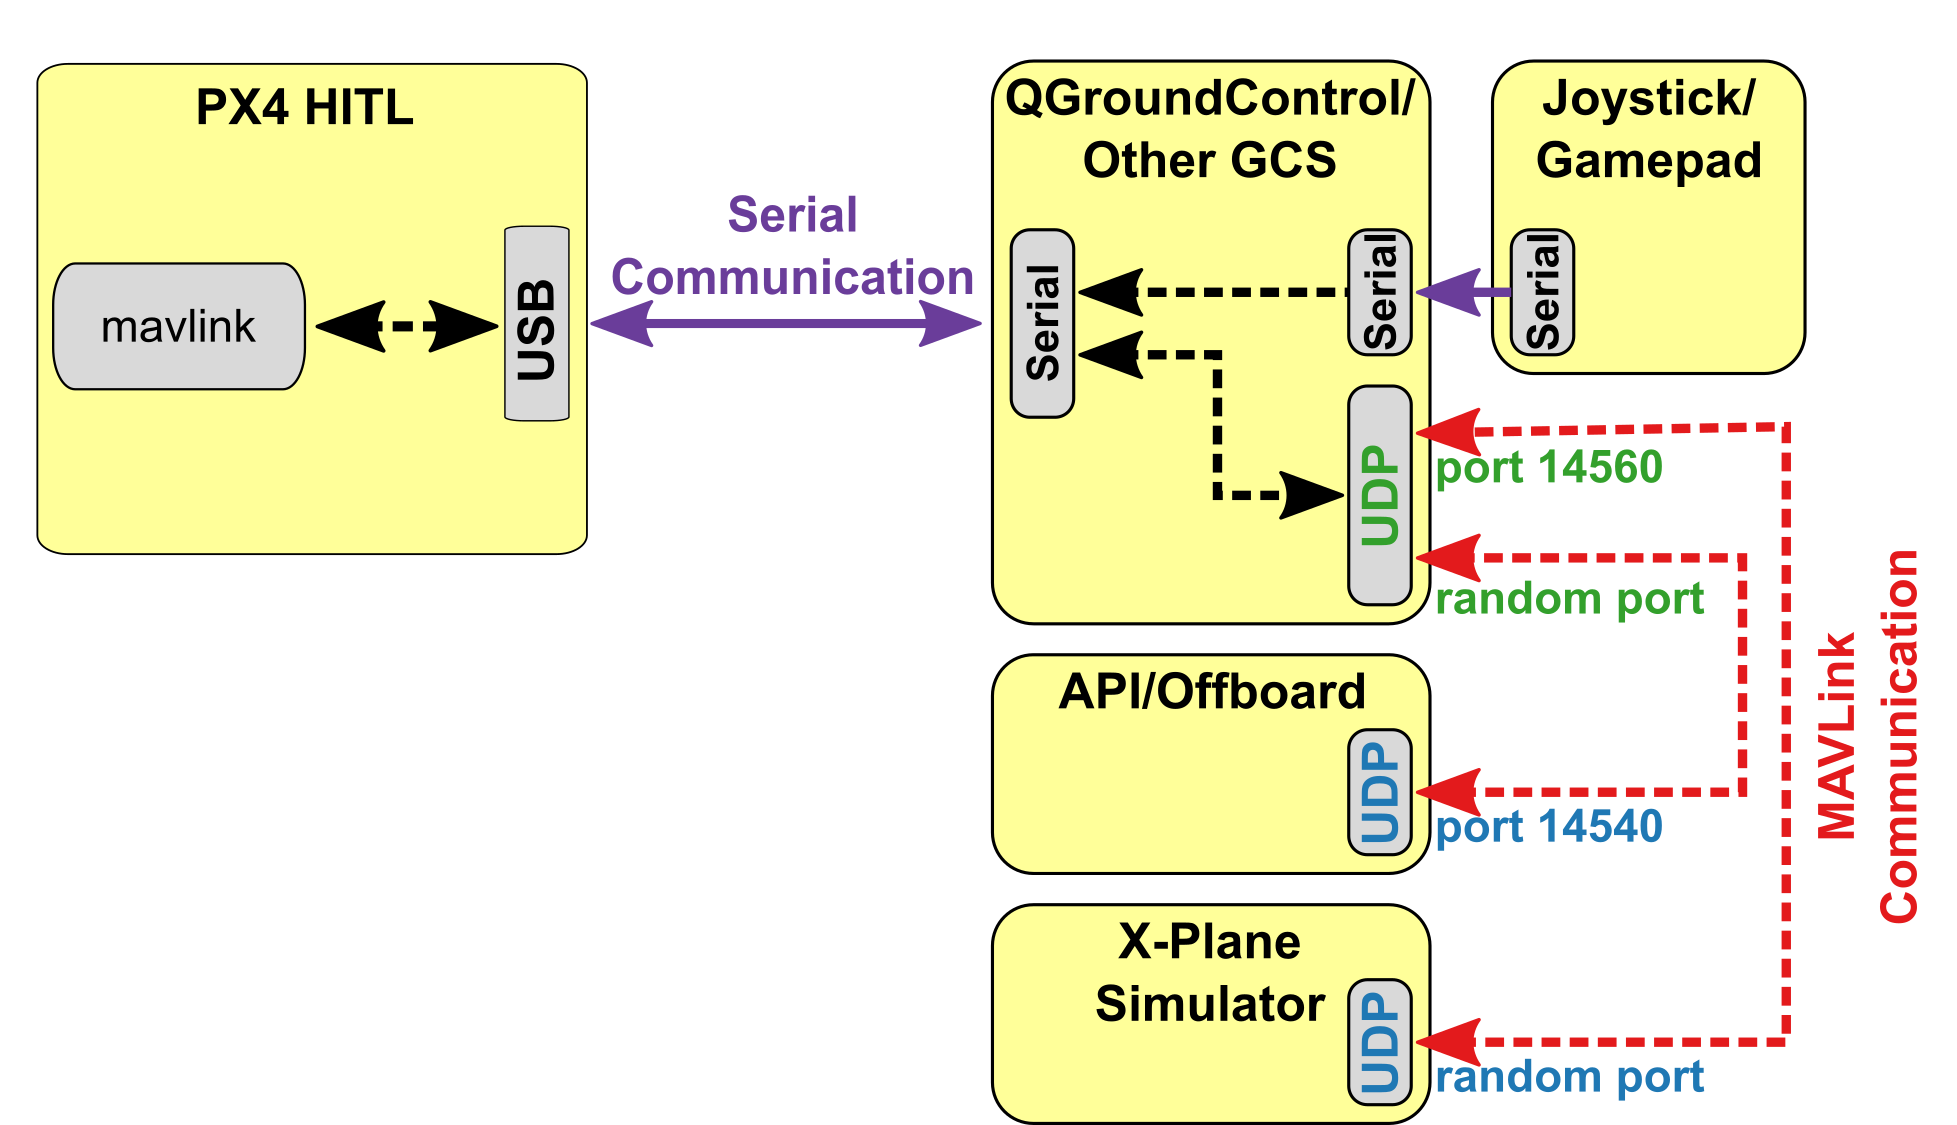
\includegraphics[width=0.8\textwidth]{picture/hitl.png}
    %   \caption{HITL-Xplane}
    % \end{figure}
    % \begin{figure}[htbp]
    %   \centering
    %   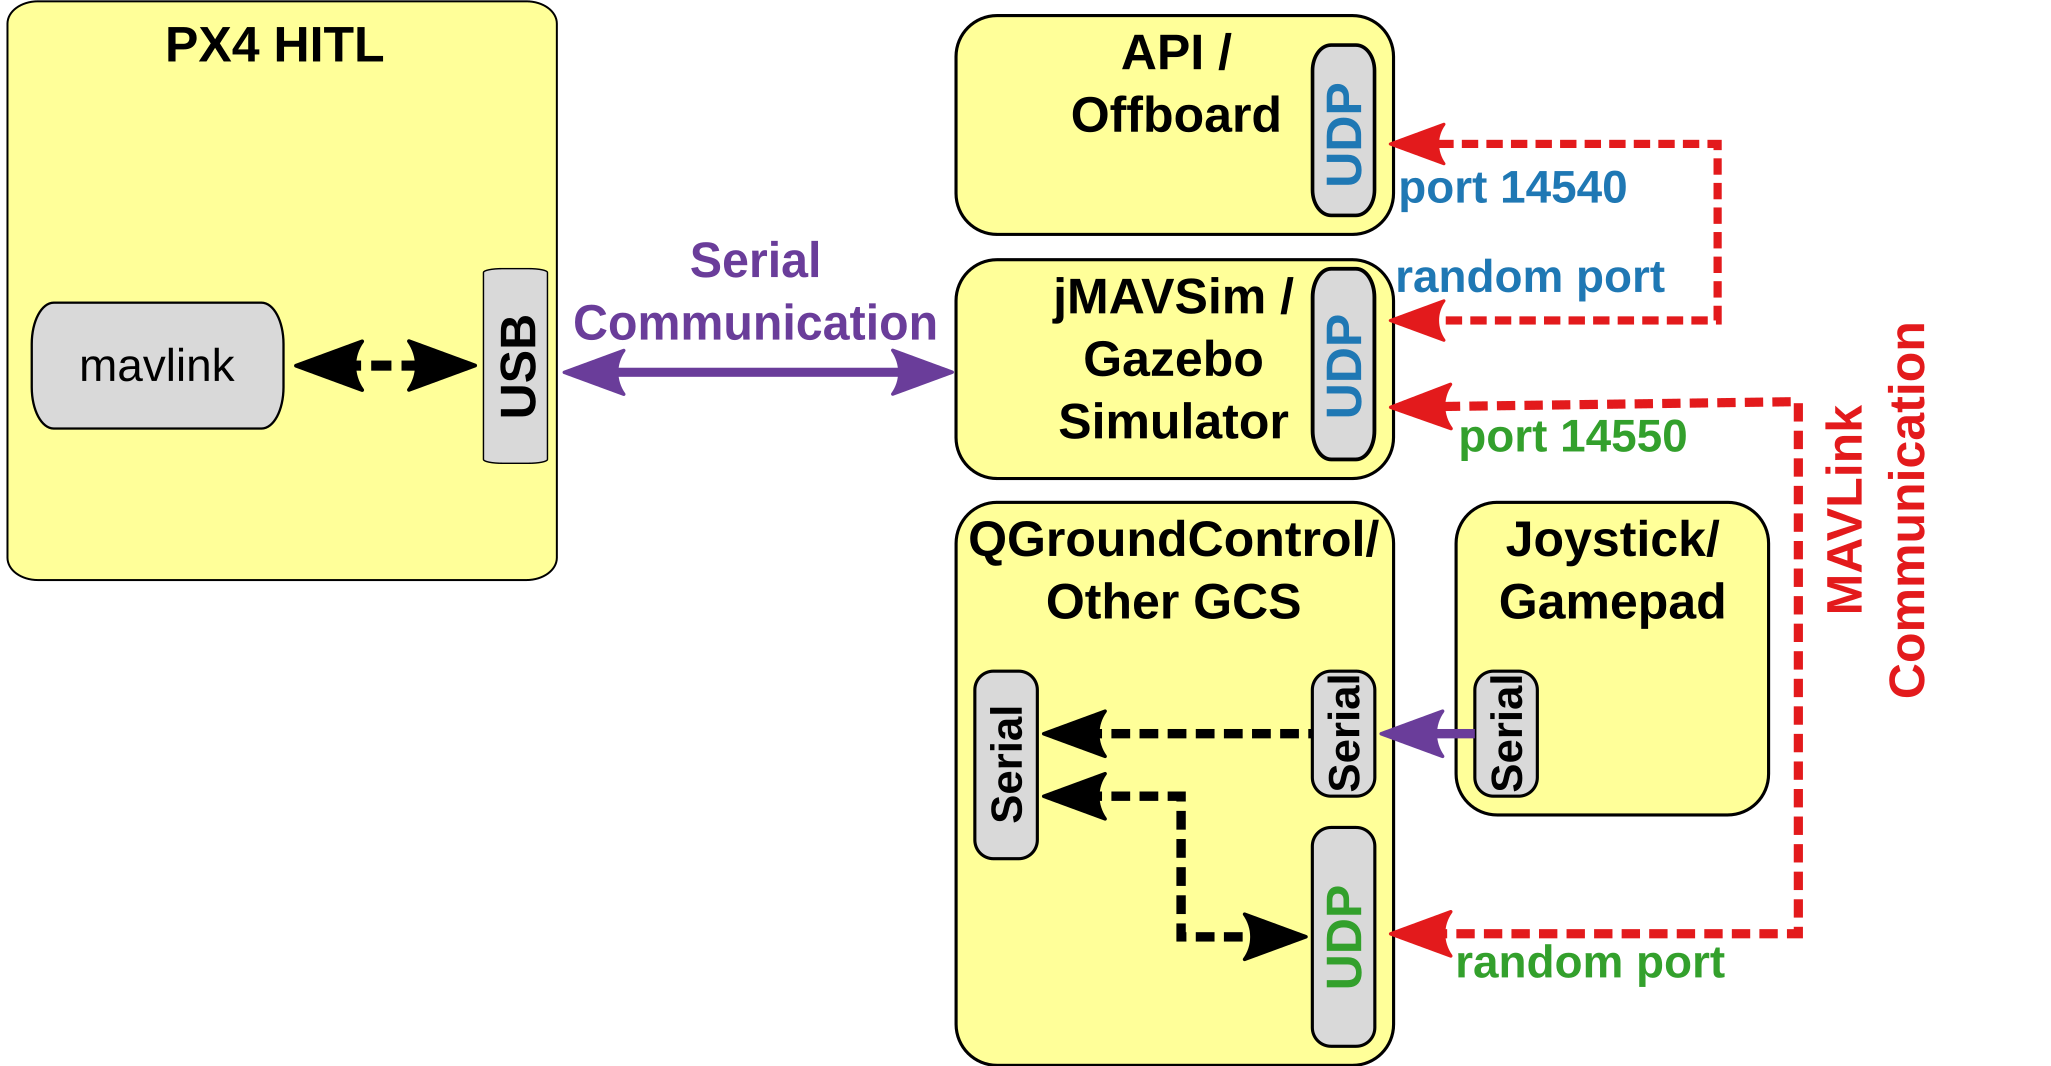
\includegraphics[width=0.8\textwidth]{picture/hitl2.png}
    %   \caption{HITL-Gazebo}
    % \end{figure}
    % \clearpage
    % \section{计算机视觉}
    %     整理一下当前的任务流.
    %   计算机视觉, 是一门研究如何对数字图像或视频进行高层语义理解的交叉学科, 赋予了机器"看"的能力, 需要实现人的大脑中(主要是视觉皮层区)的视觉能力. \par
    %   图像处理, 用计算机对图像进行分析, 已达到所需结果的技术. 图像处理一般指的是数字图像处理, 图像处理的技术一般包括图像压缩, 增强和复原, 匹配, 描述和识别三个部分. 
    %   \par 图像处理就是各种的图像变换处理, 计算机视觉在图像处理之后再识别其内部的语义, 理解视频流中的内容. 
    % \begin{figure}[htbp]
    %     \centering
    %     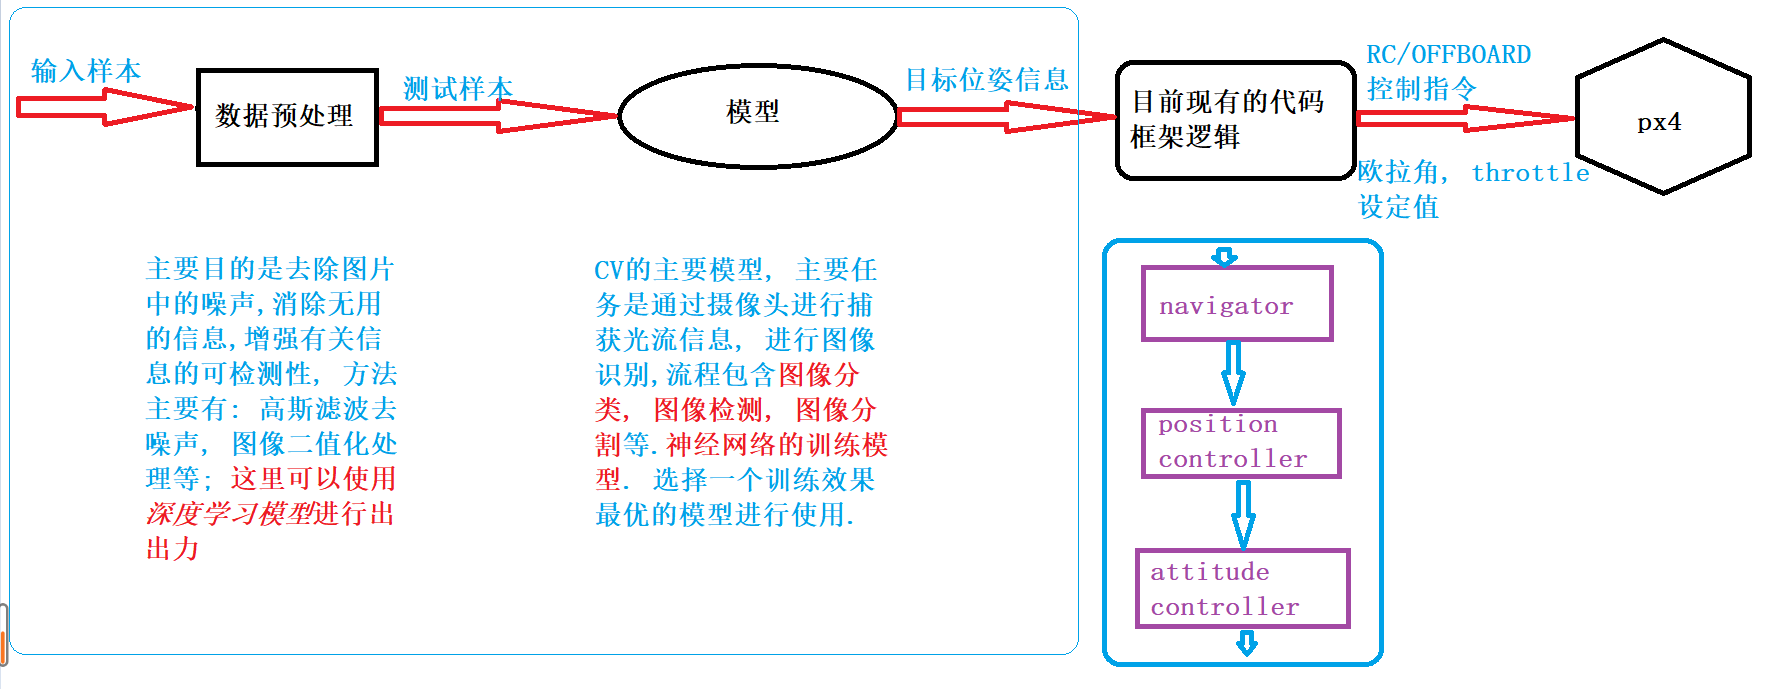
\includegraphics[width=0.8\textwidth]{picture/CV_Flow.png}
    %     \caption{CV数据流}
    % \end{figure}  
    % \clearpage
    % \section{算法内部}
    %     有时间的话细说一下代码
\end{document}

    %     \chapter{literature}
    \addcontentsline{toc}{section}{参考文献}
    \renewcommand{\refname}{参考文献}
    \begin{thebibliography}{99}
        \addtolength{\itemsep}{-2ex} % 用于更改行距
        \bibitem{1}杨玉,金敏,鲁华祥.融合简化稀疏A*算法与模拟退火算法的无人机航迹规划[J].计算机系统应用,2019,28(4):25-31. DOI:10.15888/j.cnki.csa.006864.
        \bibitem{2}张岳平,朱力超,孙涛.用Hopfield神经网络与模拟退火算法求解UAV航路规划问题[J].海军航空工程学院学报,2007,22(4):451-453,466. DOI:10.3969/j.issn.1673-1522.2007.04.012.
        \bibitem{3}赵梵喆,林跃,杨永琪.基于多目标规划的无人机路径规划[J].价值工程,2020,39(9):208-210.
        \bibitem{4}谭若晨.基于Multi-Agent系统的多UAV实时路径规划研究与实现[D].四川:电子科技大学,2013. DOI:10.7666/d.D772105.
        \bibitem{5}耿兴元.基于GPS与GIS的导航系统研究与开发[D].浙江:浙江大学,2004.
        \bibitem{6}张帅, 李学仁, 张鹏, 等.基于改进 A* 算法的无人机航迹规划[J] .飞行力学, 2016, 34( 3) : 39-43.
        \bibitem{7}Liu LF, Shi RX, Li SD, et al. Path planning for UAVS based
        on  improved  artificial  potential  field  method  through
        changing  the  repulsive  potential  function.  Proceedings  of
        2016  IEEE  Chinese  Guidance,  Navigation  and  Control
        Conference  (CGNCC).  Nanjing,  China.  2016.  2011–2015.
        \bibitem{8}D. R. Nelson, D. B. Barber, T. W. McLain and R. W. Beard, "Vector field path following for small unmanned air vehicles," 2006 American Control Conference, Minneapolis, MN, 2006, pp. 7 pp.-, doi: 10.1109/ACC.2006.1657648.
        \bibitem{9}Randal W. Beard and Timothy W. McLain, "Small Unmanned Aircraft: Theory and Practice", 2012, Princeton University Press
        \bibitem{10}R. W. {Beard} and T. W. {McLain} and D. B. {Nelson} and D. {Kingston} and D. {Johanson}, "Decentralized Cooperative Aerial Surveillance Using Fixed-Wing Miniature {UAVs}", 2006, Proceedings of the IEEE, 94, 7, 1306-1324
        \bibitem{11}R. W. {Beard} and J. {Ferrin} and J. {Humpherys}, "Fixed Wing {UAV} Path Following in Wind With Input Constraints", 2014, IEEE Transactions on Control Systems Technology, 2014, 22, 6, 2103-2117
        \bibitem{12}S. {Fari} and X. {Wang} and S. {Roy} and S. {Baldi}, "Addressing Unmodelled Path-Following Dynamics via Adaptive Vector Field: a {UAV} Test Case", 2019, IEEE Transactions on Aerospace and Electronic Systems, 10.1109/TAES.2019.2925487
    \end{thebibliography}  

\end{document}
